% Тип документа
\documentclass[a4paper,12pt]{extarticle}

% Шрифты, кодировки, символьные таблицы, переносы
\usepackage{cmap}
\usepackage[T2A]{fontenc}
\usepackage[utf8x]{inputenc}
\usepackage[russian]{babel}

% Это пакет -- хитрый пакет, он нужен но не нужен
\usepackage[mode=buildnew]{standalone}

\usepackage
	{
		% Дополнения Американского математического общества (AMS)
		amssymb,
		amsfonts,
		amsmath,
		amsthm,
		physics,
		% misccorr,
		% 
		% Графики и рисунки
		wrapfig,
		graphicx,
		subcaption,
		float,
		tikz,
		tikz-3dplot,
		caption,
		csvsimple,
		color,
		booktabs,
		pgfplots,
		pgfplotstable,
		geometry,
		% 
		% Таблицы, списки
		tabularx,
		makecell,
		multirow,
		indentfirst,
		%
		% Интегралы и прочие обозначения
		ulem,
		esint,
		esdiff,
		% 
		% Колонтитулы
		fancyhdr,
	}  

\usepackage{xcolor}
\usepackage{hyperref}

 % Цвета для гиперссылок
\definecolor{linkcolor}{HTML}{000000} % цвет ссылок
\definecolor{urlcolor}{HTML}{799B03} % цвет гиперссылок
 
\hypersetup{pdfstartview=FitH,  linkcolor=linkcolor,urlcolor=urlcolor, colorlinks=true}
% Обводка текста в TikZ
\usepackage[outline]{contour}

% Увеличенный межстрочный интервал, французские пробелы
\linespread{1.3} 
\frenchspacing 

 
\usetikzlibrary
	{
		decorations.pathreplacing,
		decorations.pathmorphing,
		patterns,
		calc,
		scopes,
		arrows,
		fadings,
		through,
		shapes.misc,
		arrows.meta,
		3d,
		quotes,
		angles,
		babel
	}


\tikzset{
	force/.style=	{
		>=latex,
		draw=blue,
		fill=blue,
				 	}, 
	%				 	
	axis/.style=	{
		densely dashed,
		blue,
		line width=1pt,
		font=\small,
					},
	%
	th/.style=	{
		line width=1pt},
	%
	acceleration/.style={
		>=open triangle 60,
		draw=magenta,
		fill=magenta,
					},
	%
	inforce/.style=	{
		force,
		double equal sign distance=2pt,
					},
	%
	interface/.style={
		pattern = north east lines, 
		draw    = none, 
		pattern color=gray!60,
					},
	cross/.style=	{
		cross out, 
		draw=black, 
		minimum size=2*(#1-\pgflinewidth), 
		inner sep=0pt, outer sep=0pt,
					},
	%
	cargo/.style=	{
		rectangle, 
		fill=black!70, 
		inner sep=2.5mm,
					},
	%
	caption/.style= {
		midway,
		fill=white!20, 
		opacity=0.9
					},
	%
	}

\newenvironment{tikzpict}
    {
	    \begin{figure}[htbp]
		\centering
		\begin{tikzpicture}
    }
    { 
		\end{tikzpicture}
		% \caption{caption}
		% \label{fig:label}
		\end{figure}
    }


\newcommand{\vbLabel}[3]{\draw ($(#1,#2)+(0,5pt)$) -- ($(#1,#2)-(0,5pt)$) node[below]{#3}}
\newcommand{\vaLabel}[3]{\draw ($(#1,#2)+(0,5pt)$) node[above]{#3} -- ($(#1,#2)-(0,5pt)$) }

\newcommand{\hrLabel}[3]{\draw ($(#1,#2)+(5pt,0)$) -- ($(#1,#2)-(5pt,0)$) node[right, xshift=1em]{#3}}
\newcommand{\hlLabel}[3]{\draw ($(#1,#2)+(5pt,0)$) node[left, xshift=-1em]{#3} -- ($(#1,#2)-(5pt,0)$) }



\newcommand\zi{^{\,*}_i}
\newcommand\sumn{\sum_{i=1}^{N}}

\tikzset{
	coordsys/.style={scale=1.8,x={(1.1cm,-0cm)},y={(0.5cm,1cm)}, z={(0cm,0.8cm)}},
	coordsys/.style={scale=1.5,x={(0cm,0cm)},y={(1cm,0cm)}, z={(0cm,1cm)}}, 
	coordsys/.style={scale=1.5,x={(1cm,0cm)},y={(0cm,1cm)}, z={(0cm,0cm)}}, 
}

\usepgfplotslibrary{units}


% Draw line annotation
% Input:
%   #1 Line offset (optional)
%   #2 Line angle
%   #3 Line length
%   #5 Line label
% Example:
%   \lineann[1]{30}{2}{$L_1$}

\newcommand{\lineann}[4][0.5]{%
    \begin{scope}[rotate=#2, blue,inner sep=2pt, ]
        \draw[dashed, blue!40] (0,0) -- +(0,#1)
            node [coordinate, near end] (a) {};
        \draw[dashed, blue!40] (#3,0) -- +(0,#1)
            node [coordinate, near end] (b) {};
        \draw[|<->|] (a) -- node[fill=white, scale=0.8] {#4} (b);
    \end{scope}
}

\newcommand{\lineannn}[4][0.5]{%
    \begin{scope}[rotate=#2, blue,inner sep=2pt, ]
        \draw[dashed, blue!40] (0,0) -- +(0,#1)
            node [coordinate, near end] (a) {};
        \draw[dashed, blue!40] (#3,0) -- +(0,#1)
            node [coordinate, near end] (b) {};
        % \draw[color=white, color=blue] (a) -- node[fill=white, scale=0.8] {#4} (b);
        \draw[->|] (a)++(-0.3,0) -- (a);
        \draw[->|] (b)++(0.3,0) coordinate (xx) -- (b);
        \draw (xx) node[fill=white, scale=0.8, right] {#4};
    \end{scope}
}

% Круговая стрелка относительно центра (дуга из центра)
\tikzset{
  pics/carc/.style args={#1:#2:#3}{
    code={
      \draw[pic actions] (#1:#3) arc(#1:#2:#3);
    }
  },
  dash/.style={
  	dash pattern=on 5mm off 5mm
  }
}

% Среднее <#1>
\newcommand{\mean}[1]{\langle#1\rangle}

\pgfplotsset{
    % most recent feature set of pgfplots
    compat=newest,
}

% const прямым шрифтом
\newcommand\ct[1]{\text{\rmfamily\upshape #1}}
\newcommand*{\const}{\ct{const}}


\usepackage[europeanresistors,americaninductors]{circuitikz}

% Style to select only points from #1 to #2 (inclusive)
\pgfplotsset{select/.style 2 args={
    x filter/.code={
        \ifnum\coordindex<#1\def\pgfmathresult{}\fi
        \ifnum\coordindex>#2\def\pgfmathresult{}\fi
    }
}}


\usepackage{array}
\usepackage{pstool}


%%%%%%%%%%%%%%%%%%%%%%%%%%%%%%%%%%%%%%%%%%%%%%%%%
\makeatletter
\newif\if@gather@prefix 
\preto\place@tag@gather{% 
  \if@gather@prefix\iftagsleft@ 
    \kern-\gdisplaywidth@ 
    \rlap{\gather@prefix}% 
    \kern\gdisplaywidth@ 
  \fi\fi 
} 
\appto\place@tag@gather{% 
  \if@gather@prefix\iftagsleft@\else 
    \kern-\displaywidth 
    \rlap{\gather@prefix}% 
    \kern\displaywidth 
  \fi\fi 
  \global\@gather@prefixfalse 
} 
\preto\place@tag{% 
  \if@gather@prefix\iftagsleft@ 
    \kern-\gdisplaywidth@ 
    \rlap{\gather@prefix}% 
    \kern\displaywidth@ 
  \fi\fi 
} 
\appto\place@tag{% 
  \if@gather@prefix\iftagsleft@\else 
    \kern-\displaywidth 
    \rlap{\gather@prefix}% 
    \kern\displaywidth 
  \fi\fi 
  \global\@gather@prefixfalse 
} 
\newcommand*{\beforetext}[1]{% 
  \ifmeasuring@\else
  \gdef\gather@prefix{#1}% 
  \global\@gather@prefixtrue 
  \fi
} 
\makeatother
%%%%%%%%%%%%%%%%%%%%%%%%%%%%%%%%%%%%%%%%%%%%%%%%%

\geometry		
	{
		left			=	2cm,
		right 			=	2cm,
		top 			=	3cm,
		bottom 			=	3cm,
		bindingoffset	=	0cm
	}

%%%%%%%%%%%%%%%%%%%%%%%%%%%%%%%%%%%%%%%%%%%%%%%%%%%%%%%%%%%%%%%%%%%%%%%%%%%%%%%



	%применим колонтитул к стилю страницы
\pagestyle{fancy} 
	%очистим "шапку" страницы
\fancyhead{} 
	%слева сверху на четных и справа на нечетных
\fancyhead[R]{\labauthors} 
	%справа сверху на четных и слева на нечетных
\fancyhead[L]{Отчёт по лабораторной работе №\labnumber} 
	%очистим "подвал" страницы
\fancyfoot{} 
	% номер страницы в нижнем колинтуле в центре
\fancyfoot[C]{\thepage} 

%%%%%%%%%%%%%%%%%%%%%%%%%%%%%%%%%%%%%%%%%%%%%%%%%%%%%%%%%%%%%%%%%%%%%%%%%%%%%%%

\renewcommand{\contentsname}{Оглавление}

\usepackage{tocloft}
% \renewcommand{\cftpartleader}{\cftdotfill{\cftdotsep}} % for parts
% \renewcommand{\cftsectiondotsep}{\cftdotsep}% Chapters should use dots in ToC
\renewcommand{\cftsecleader}{\cftdotfill{\cftdotsep}}
%\renewcommand{\cftsecleader}{\cftdotfill{\cftdotsep}} % for sections, if you really want! (It is default in report and book class (So you may not need it).
% ---------
% \newcommand{\cftchapaftersnum}{.}%
% \usepackage{titlesec}
% \titlelabel{\thetitle.\quad}
\usepackage{secdot}
\sectiondot{subsection}

\begin{document}

\def\labauthors{}
\def\labgroup{430}
\def\labnumber{2}
\def\labtheme{Эффект Зеемана}
\renewcommand{\vec}{\mathbf}

\renewcommand{\phi}{\varphi}
\renewcommand{\hat}{\widehat}

\begin{titlepage}

\begin{center}

{\small\textsc{Нижегородский государственный университет имени Н.\,И. Лобачевского}}
\vskip 1pt \hrule \vskip 3pt
{\small\textsc{Радиофизический факультет}}

\vfill

{\Large Отчет по лабораторной работе №\labnumber\vskip 12pt\bfseries \labtheme}
	
\end{center}

\vfill
	
\begin{flushright}
	{Выполнили студенты \labgroup\ группы\\ \labauthors}%\vskip 12pt Принял:\\ Менсов С.\,Н.}
\end{flushright}
	
\vfill
	
\begin{center}
	Нижний Новгород, \the\year
\end{center}

\end{titlepage}




\newpage
%%%%%%%%%%%%%%%%%%%%%%%%%%%%%%%%%%%%%%%%%%%%%%%%%%%%%%%%%%%%%%%%%%%%%%%
\section{Теоретическая часть}
\subsection{Введение}
%!TEX root = ../zeeman.tex
В 1896 г. Зееман обнаружил, что спектральные линии определенным образом расщепляются, если источник света поместить в магнитное поле. При наблюдении поперек поля спектральная линия расщепляется на три линейно поляризованные компоненты. Средняя компонента не смещена, крайние смещены в противоположные стороны на одинаковые расстояния (в шкале частот). Смещение пропорционально напряженности внешнего магнитного поля \textbf{B}. В средней компоненте электрический вектор направлен параллельно магнитному полю (такие компоненты называются $\pi-$компонентами), в крайних - перпендикулярно к нему(такие компоненты называются $\sigma-$компонентами). Интенсивность $\pi-$компоненты вдвое, а каждой из $\sigma-$компонент в четыре раза меньше интенсивности исходной линии. 

При наблюдении вдоль магнитного поля получается такое же смещение (при одинаковой напряженности магнитного поля), что и в предыдущем случае, но несмещенная компонента отсутствует. Интенсивность каждой компоненты вдвое меньше интенсивности исходной спектральной линии. Обе компоненты поляризованы по кругу в противоположных направлениях (их принято называть также $\sigma-$компонентами). Если свет распространяется в направлении магнитного поля, то $\sigma-$компонента с меньшей частотой поляризована по правому, с большей - по левому кругу. При изменении направления магнитного поля на противоположное меняется на противоположную и круговая поляризация обеих компонент.
 
 Описанная картина расщепления спектральных линий объясняется классической теорией Лорентца. Как и классическая теория дисперсии, это есть модельная теория, в простейшей форме которой излучающими центрами являются гармонические осцилляторы в виде квазиупругосвязанных электронов. В отсутствие внешнего магнитного поля уравнение движения таокгор электрона имеет вид $\ddot{\vec{r}}-\omega_0^2 \vec{r}=0$, где $\omega_0$ - собственная частота электрона. При наличии постоянного магнитного поля на электрон действует еще сила Лорентца $\vec{F_l}=-\frac ec[\dot{\vec{r}}, \vec{B}]$. Уравнение движения электрона принимает вид: $$\ddot{\vec{r}}-\omega_0^2 \vec{r}=-\frac{e}{mc}[\dot{\vec{r}}, \vec{B}],$$ где m - масса электрона. Введя ларморовскую частоту $$\Omega=\frac{e}{2mc}\vec{B},$$ приведем его к виду $$\ddot{\vec{r}}+2[\dot{\vec{r}},\vec{\Omega}]+\omega_0^2\vec{r}=0.$$
 Классическая теория сводится к решению этого уравнения. Перейдем к системе трех скалярных уравнений $$\ddot{x}+2\Omega \dot{x}+\omega_0^2x=0,$$ $$\ddot{y}+2\Omega \dot{y}+\omega_0^2y=0,$$ $$\ddot{z}+\omega_0^2z=0.$$
Из последнего уравнения видно, что магнитное поле не влияет на движение электрона вдоль магнитного поля. Это и понятно, так как при таком движении не возникает силы, действующей со стороны магнитного поля. Интегрирование двух первых уравнений удобно провести в комплексной форме. Объединим: $\zeta=x+iy$, $-i\dot{\zeta}=\dot{y}-i\dot{x}$, умножим второе уравнение на i и сложим с первым. Тогда $$\ddot{\zeta}-i2\Omega\dot{\zeta}+\omega_0^2\zeta=0.$$Ищем решение уравнения  в виде $\zeta=e^{i\omega t}$. Постоянная $\omega$ найдется из квадратного уравнения $\omega^2+2\Omega \omega+\omega_0^2=0,$ которое дает $$\omega=\Omega \pm \sqrt{\omega_0^2+\Omega^2}.$$ Даже в очень сильных магнитных полях квадратом ларморовской частоты можно пренебречь по сравнению с $\omega_o^2$. С большой точностью $\omega=\pm \omega_0+\Omega$. Переобозначим: $\omega_1=\omega_0+\Omega$, $\omega_2=\omega_0-\Omega$. Тогда $$\zeta_1=e^{i\omega_1 t}, \zeta_2=e^{i\omega_2 t}.$$

\begin{figure}[h]
	\centering
	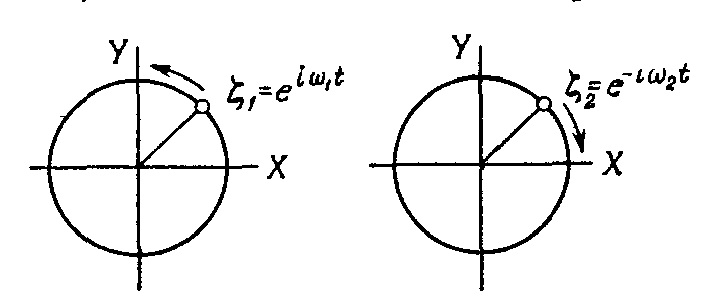
\includegraphics[width=0.4\linewidth]{fig/fig11}
\end{figure}

Первое решение представляет круговое движение, в котором электрон вращается против часовой стрелки с угловой частотой $\omega_1$, второе - также круговое движение, но по часовой стрелке и с частотой $\omega_2$. Общее решение соответствует наложению таких двух вращений и представляется в виде $\zeta=C_1\zeta_1+C_2\zeta_2$, где $C_1$ и $C_2$ - произвольные постоянные.

Согласно квантовой теории излучения энергия атома $E$ может принимать лишь дискретные строго определенные значения. Совокупность таких разрешенных значений (уровней энергии) называют \textbf{энергетическим спектром атома}. Энергетический спектр атома может быть задан с помощью вполне определенного набора внутренних характеристик атома - его \textbf{квантовых чисел}. Наиболее точный смысл каждого квантового числа выясняется при решении \textbf{уравнения Шредингера}, в котором квантовые числа определяют \textbf{спектр собственных значений}. Мы же введем лишь названия и обозначения, а там, где это возможно, дадим краткую, более или менее наглядную и нс слишком строгую, характеристику квантовых чисел атома:

$n$ -- \textbf{главное квантовое число}, определяющее среднее расстояние электронного облака от ядра;

$L$ -- \textbf{орбитальное квантовое число}, характеризующее сумму моментов импульса электронов $\vec{P_L}$, связанных с их вращением вокруг ядра;

$S$ -- \textbf{спиновое квантовое число}, описывающее сумму собственных моментов импульса электронов $\vec{P_S}$, не связанных с их вращением вокруг ядра\footnote{Наличие собственною механического момента (спина) и магнитного момента у покоящегося электрона не имеет удовлетворительного наглядного толкования и должно восприниматься как факт, однозначно следующий из результатов многочисленных экспериментов.};

$J$ -- \textbf{азимутальное квантовое число}, которому ставится в соответствие полный механический момент электронов в атоме:

\begin{equation}
	\vec{P_J}=\vec{P_L}+\vec{P_S}
	\label{eq:1}
\end{equation}

$M_J$ -- \textbf{магнитное квантовое число}, название которого связано с тем, что энергия атома зависит от $M_J$ лишь при наличии внешнего магнитного поля: $E(n,J,L,S,M_J)$. В отсутствии магнитного поля для всех допустимых значений $M_J$ энергия атома имеет одно и то же значение $E(n,J,L,S,M_J)$ -- в этом случае говорят, что имеет место \textbf{вырождение} (неоднозначность) состояния атома по квантовому числу $M_J$. Из элементарной физики известно, что в магнитном поле могут изменить свою энергию лишь системы, имеющие (или приобретающие) \textbf{магнитный момент} $\vec{\mu}$, причем изменение энергии равно:

\begin{equation}
	\delta E=-(\vec{\mu}\vec{H})=-\mu_HH.
	\label{eq:2}
\end{equation}

Из сказанного ясно, что квантовое число $M_J$ характеризует проекцию магнитного момента атома $\vec{\mu}$ на направление внешнего магнитного поля $\vec{H}$.

\begin{figure}[tb]
	\centering
	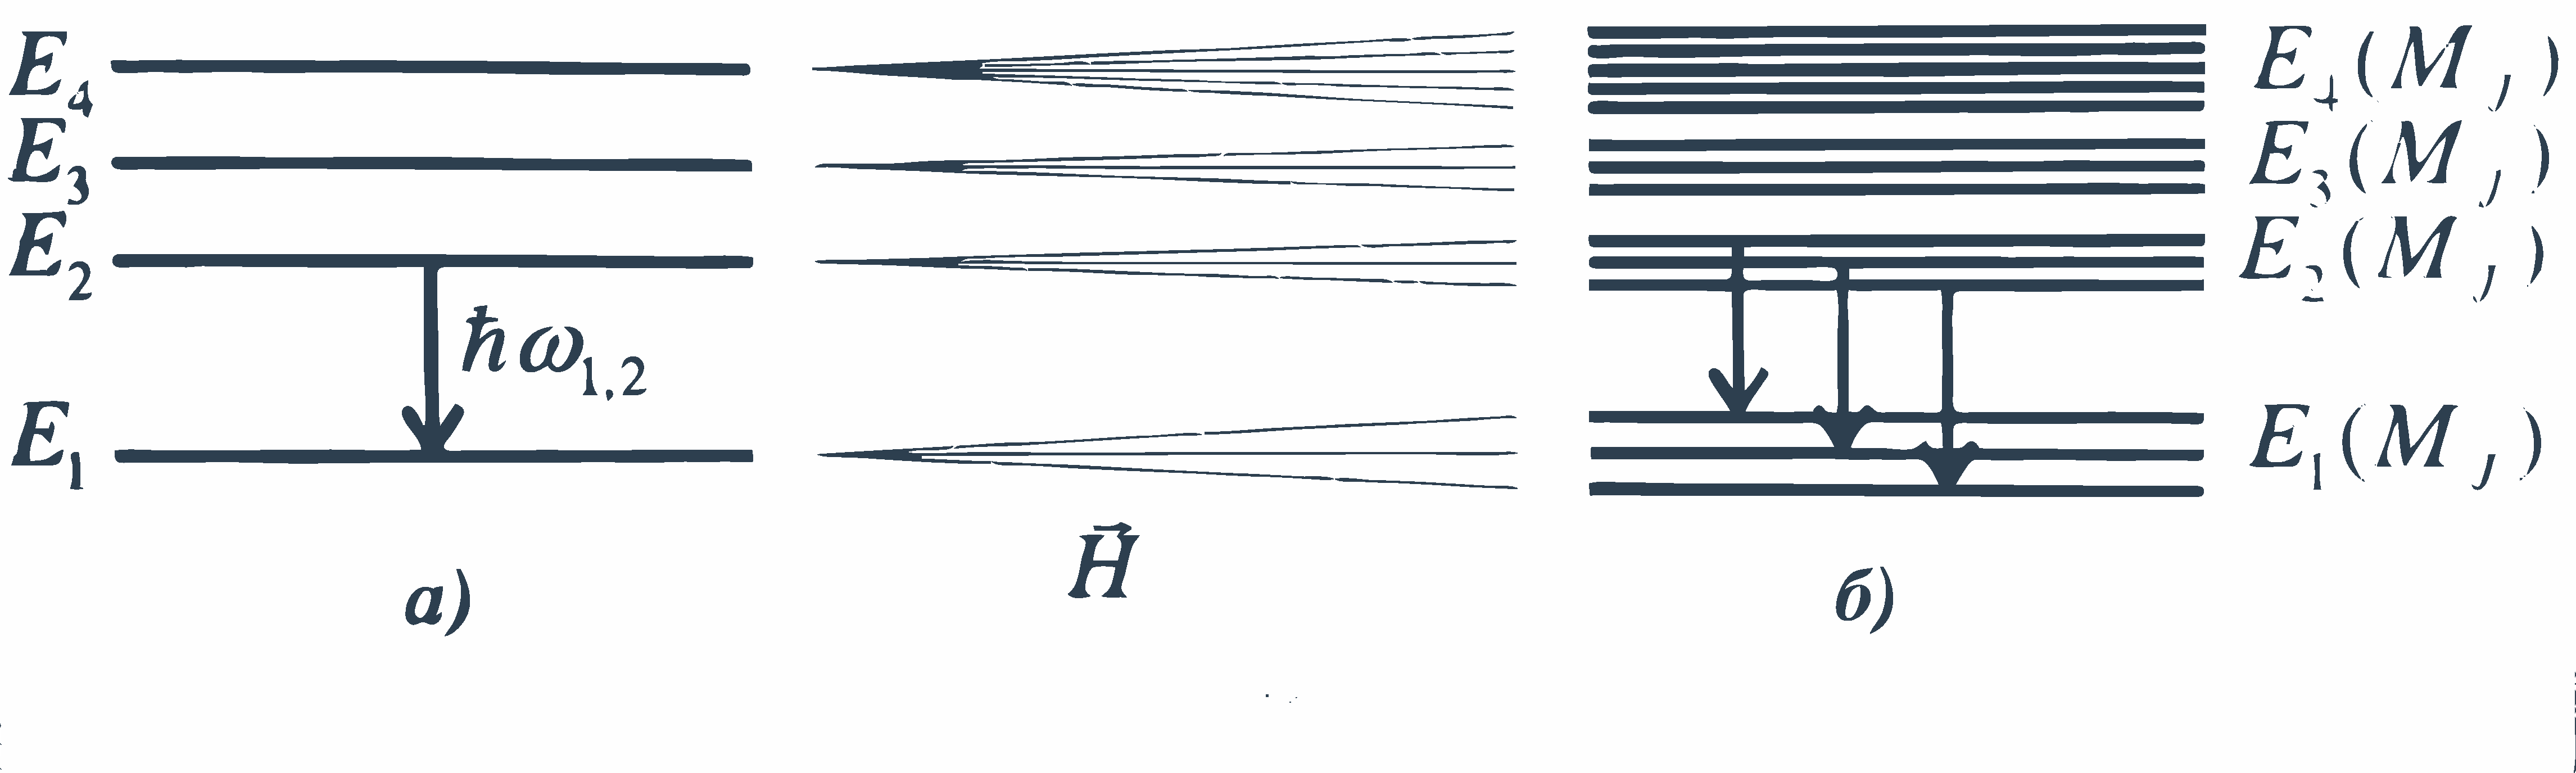
\includegraphics[width=\linewidth]{fig/fig1}
	\caption{Энергетическая структура атома и некоторые из возможных излучательных переходов
	а) в невозмущенном состоянии, б) при наложении внешнего магнитного поля}
	\label{fig:1}
\end{figure}

При переходе атома с более высокого энергетического уровня $E_2$ на более низкий $E_1$, излучается квант электромагнитной энергии (\ref{fig:1}) с частотой

\begin{equation}
\omega_{1,2}=\frac{E_2-E_1}{\hbar}
\label{eq:3}
\end{equation}
где $\hbar = 1.054\cdot10^{-27}$ эрг$\cdot$с -- постоянная Планка. Поскольку при наложении внешнего магнитного поля вырождение энергетических состояний $E_2$ и $E_1$ по квантовому числу $M_J$ снимается (т.е. происходит расщепление каждого энергетического уровня на несколько подуровней), в спектре излучения мы вместо одной наблюдаем несколько частот (линий) излучения (\ref{fig:1}). Этот эффект расщепления спектральных линий атомов в магнитном поле и называется \textbf{эффектом Зеемана}.

Точное решение уравнение Шредингера может быть найдено лишь в небольшом числе простейших случаев. Предположим, что гамильтониан данной физической системы имеет вид:
$$\widehat{H}=\widehat{H_0}+\widehat{V},$$
где $\widehat{V}$ представляет собой малую поправку к "невозмущенному" оператору $\widehat{H_0}$. Рассматриваются возмущения, не зависящие явно от времени.

Задача теории возмущений для дискретного спектра может быть сформулирована следующим образом. Предполагается, что собственные функции $\psi_n^{(0)}$ и собственные значения оператора $\widehat{H_0}$ известны, т.е известны точные решения уравнения

$$\widehat{H_0}\psi^{(0)}=E^{(0)}\psi{(0)}.$$

Требуется найти приближенные значения уравнения

$$\widehat{H}\psi=(\widehat{H_0}+\widehat{V})\psi=E\psi,$$
т.е приближенные выражения для собственных функций $\psi_n$ и значений $E_n$ возмущенного оператора $\widehat{H}$. Все собственные значения оператора $\widehat{H_0}$ не вырождены.

Разложим искомую функцию $\psi$ по функциям $\psi^{(0)}_m$:

$$\psi=\sum_m C_m \psi^{(0)}_m.$$

$$\sum_m C_m(E_m^{(0)}+\widehat{V})\psi_m^{(0)}=\sum_m C_mE\psi_m^{(0)},$$
умножив равенство с обеих сторон на $\psi_k^{(0)*}$ и интегрируя:

$$(E-E_k^{(0)})C_k=\sum_m V_{km}C_m.$$

Здесь введена матрица $V_{km}$ оператора возмущения $\widehat{V}$, определенная с помощью невозмущенных функций $\psi_m^{(0)}$:

$$V_{km}=\int \psi_k^{(0)*} \widehat{V} \psi_m^{(0)} dq.$$
будем искать значения коэффициентов $C_m$ и энергии Е в виде рядов

$$E=E^{(0)}+E^{(1)}+E^{(2)}+..., C_m=C_m^{(0)}+C_m^{(1)}+C_m^{(2)}+...,$$
где величины $E^{(1)}, C_m^{(1)}$ - того же порядка малости, что и возмущение $\widehat{V}$, величины $E^{(2)}, C_m^{(2)}$ - второго порядка малости и т.д. 

Определим поправки к n-му собственному значению и собственной функции, соответственно чему полагаем $C_n^{(0)}=1, C_m^{(0)}=0, m\neq n$. Для отыскания первого приближения учтем, что $E=E_n^{(0)}+E_n^{(1)}, C_k=C_k^{(0)}+C_k^{(1)}$, сохранив только члены первого порядка. Уравнение с $k=n$ дает:

$$E_n^{(1)}=V_{nn}=\int \psi_k^{(0)*} \widehat{V} \psi_n^{(0)} dq.$$

Таким образом, поправка первого приближения к собственному значению $E_n^{(0)}$ равна среднему значению возмущения в состоянии $\psi_n^{(0)}$. 

При $k\neq n$: $C_k^{(1)}=\frac{V_{kn}}{E_n^{(0)}-E_k^{(0)}}$, a $C_n^{(1)}$ остается произвольным и должно быть выбрано так, чтобы функция $\psi_n=\psi_n^{(0)}+\psi_n^{(1)}$ была нормирована с точностью до членов первого порядка включительно. Для этого надо положить $C_n^{(1)}=0$. Действительно, функция
$$\psi_n^{(1)}=\sum_{m,m\neq n} \frac{V_{mn}}{E_n^{(0)}-E_m^{(0)}}\psi_m^{(0)}$$
ортогональна к $\psi_n^{(0)}$, а поэтому интеграл от $|\psi_n^{(0)}-\psi_n^{(1)}|^2$ отличается от единицы лишь на величину второго порядка малости. Так определяется поправка первого приближения к волновым функциям.

Должно иметь место  неравенство

$$|V_{mn}|\ll|E_n^{(0)}-E_m^{(0)}|,$$
т.е матричные элементы возмущения должны быть малы по сравнению с соответствующими разностями невозмущенных уровней энергии.

Определим еще поправку второго приближения к собственному значению $E_n^{(0)}$. Для этого полагаем $E=E_n^{(0)}+E_n^{(1)}+E_n^{(2)}, C_k=C_k^{(0)}+C_k^{(1)}+C_k^{(2)}$ и рассматриваем члены второго порядка малости. Уравнение с $k=n$ дает

$$E_n^{(2)}C_n^0=\sum_{m,m\neq n} V_{nm}C_m^{(1)},$$
откуда

$$E_n^{(2)}=\sum_{m,m\neq n} \frac{|V_{mn}|^2}{E_n^{(0)}-E_m^{(0)}}$$
(воспользовались тем, что в силу эрмитовости оператора $\widehat{V}: V_{mn}=V_{nm}^*$).

Отметим, что поправка второго приближения к энергии нормального состояния всегда отрицательна. Если $E_n^{(0)}$ соответствует наименьшему значению, то все члены в сумме отрицательны.

Дальнейшие приближения можно вычислить аналогичным образом.

\subsection{Феноменологический расчет зеемановского расщепления}
%!TEX root = ../zeeman.tex
С математической точки зрения квантовые числа \textbf{\textsl{ L,S,J}} определяют собственные значения уравнения Шредингера $\mathbf{\mathit{P_L,P_S,P_J}}$ 
для \textbf{волновой функции} электронов $\Psi$ в центрально - симметричном поле ядра, а дискретность собственых значений связана с тем, что волновая функция должна однозначно описывать состояние электронного облака в данной точке, то есть быть периодической функцией угла:

\begin{equation}
\Psi(\Theta+2\pi)=\Psi(\Theta)
\label{eq:4} 
\end{equation}

Условие (\ref{eq:4}) приводит к следующемму \textbf{правилу квантования} проекции момента импульса на фиксированное направление (например, на направление $\vec{H}$):

\begin{equation}
P_{J_H} = \hbar M_J
\label{eq:5} 
\end{equation}

где квантовое число $M_{J}$ принимает $2J+1$ значений: $J,J-1,..0,...-J$.  При этом модуль момента импульса равен: 

\begin{equation}
P_{J}=\hbar \sqrt {J(J+1)}
\label{eq:6} 
\end{equation}

Квантовое число $J$ в силу различной возможной ориентации векторов $\vec P_S$ (см. формулу (\ref{eq:1})) принимает следующие значения: $$J=L+S,L+S-1,...,|L-S|.$$

Для расчета зеемановского расщепления по формулам (\ref{eq:2}),(\ref{eq:3}) необходимо связать вычисленный по формуле (\ref{eq:6}) полный механический момент атома со средней проекцией 
$\mu_H$ его магнитного момента на направление $\vec H$. Вид этой связи зависит от квантового состояния атома, а ее вычисление представляет собой отдельную задачу, решение которой будет дано в п.3 в достаточно простом приближении. Пока же для получения общей формулы зеемановского расщепления представим связь $\mu_H$ и $P_J$ феноменологически в виде: 

\begin{equation}
\mu_{H}=\mu_{0} g \frac{P_{J_H}}{\hbar}=\mu_{0} g M_{J},
\label{eq:7} 
\end{equation}

где \textbf{g} - так называемый \textbf{фактор} (или \textbf{множитель}) \textbf{Ланде} соответствующего квантового состояния, а величина $\mu_0$ называется \textbf{магнетоном Бора} и имеет смысл наименьшей отличной от нуля проекции магнитного момента, связанного с орбитальным движением электрона в атоме: 
$\displaystyle{\mu_{0} = {\frac{e\hbar}{2mc}}=9.27\cdot10^{-21}}$
эрг/Гс.
Здесь и далее: e - элементарный заряд, m - масса электрона, с - скорость света.

Будем считать, что внешнее магнитное поле достаточно слабо, так что $\mu_0 H$ много меньше разности энергий между любой парой  рассматриваемых уровней атома. Тогда зеемановское расщепление интересующего нас уровня $E$ можно рассматривать изолированно и в соответствии с (\ref{eq:2}), (\ref{eq:5}) и (\ref{eq:7}) написать: 
\begin{equation}
\mathbf{\delta E_{M} = - g \mu_{0} H M_J}.
\label{eq:8} 
\end{equation}  

Таким образом, при переходе между каждой парой подуровней, образовавшихся в результате расщепления в магнитном поле энергетических состояний, описываемых квантовыми числами $(n_{2},J_{2},L_{2},S_{2})$ и $(n_{1},J_{1},L_{1},S_{1})$  будут излучать частоты: 
\begin{equation}
\omega_{1,2} = \frac{E_{2}(n_{2},J_{2},L_{2},S_{2},M_{J_{2}})-E_{1}(n_{1},J_{1},L_{1},S_{1},M_{J_1})}{\hbar}
\label{eq:9} 
\end{equation}


Однако не все из указанных переходов могут быть осуществлены. Действительно, так как квант электромагнитного излучения (фотон) имеет отличный от нуля собственный момент импульса (спин) $P_{\mu_H} = {0,\pm\hbar}$, то из закона сохранения момента импульса и формулы (\ref{eq:5}) следует, что в процессе излучения магнитное квантовое числоа $M_J$ атома  может либо измениться на удиницу ($\Delta M=\pm 1$),  либо остаться еизменным ($\Delta M = 0$) . Можно показать, что аналогичные ограничения накладываются на изменение квантового числа $J$ : $\Delta J = {0,\pm 1}$.

Указанные усдлвия носят название правил отбора и определяют допустимые переходы медлу щеемановскими уровнями. Соответствующие им зеемановские линии в спектре излучения носят название $\mathbf{\pi}$ - (при $\Delta M = 1$) и $\mathbf{\sigma }$ - (при $\Delta M= \pm 1$)  компонент и отличаются, в частности, поляризацией. Вдоль магнитного поля излучаются лишь циркулярно поляиризованные $\sigma$ - компоненты,  поляризованные линейно в перпендикулярных друг другу плоскостях. В зависимости от направления наблюдения говорят соответственно о \textbf{продольном} и \textbf{поперечном} \textit{эффекте Зеемана}. 

Приведенные выше формулы позволяют легко рассчитать вид зеемановского спектра. Пусть в отсутствие внешнего магнитного поля при переходе между уровнями $E_{1}(J_{1},L_{1},S_{1})$ и $E_{2}(J_{2},L_{2},S_{2})$, которые далее будем называть \textbf{комбинирующими}, излучается линия с частотой $\omega_0$. При наложении поля расщепления каждого из комбинирующих уровней будет определяться формулой (\ref{eq:8}), и в соответствии с правилами отбора в системе станут возможны переходы между уровнями с квантовыми числами: 

$$(J_{1},L_{1},S_{1},M)\rightarrow(J_{2},L_{2},S_{2},M)$$
$$(J_{1},L_{1},S_{1},M \pm1)\rightarrow(J_{2},L_{2},S_{2},M)$$
с излучением частот $\omega_{M_1,M_2}$
$$\omega_{M2,M1}=\frac{E_{M2}-E_{M1}}{\hbar}$$
$$\omega_0=\frac{E_{02}-E_{01}}{\hbar}$$
$$E_1=E_{01}-(\vec{\mu},\vec{H})=E_{01}-M_{J1}\mu_0g_1H$$
$$E_2=E_{02}-(\vec{\mu},\vec{H})=E_{02}-M_{J2}\mu_0g_2H$$


\begin{equation} \tag{10a}
	\omega_{M2,M1}=\frac{E_{02}-M_{J2}\mu_0g_2H-E_{01}+M_{J1}\mu_0g_1H}{\hbar}=\omega_0+\frac{h\mu_0}{\hbar}(M_{J1}g_1-M_{J2}g_2)
	\label{eq:10a} 
\end{equation}
\begin{equation} \tag{10b}
	\omega_{M_{\pm1},M}=\omega_0 + \frac{\delta E_{1,M\pm1} - \delta E_{2,M}}{\hbar} = \omega_0 \pm g_1 \frac {\mu_0 H}{\hbar} +(g_1 - g_2)M\frac{\mu_0 H}{\hbar} 
	\label{eq:10b} 
\end{equation}
смещенных относительно основной частоты $\omega_0$ на величину:
	\begin{equation}
	\addtocounter{equation}{1}
	\Delta \omega_{M_1,M_2} = \omega_{M_1,M_2} - \omega_{0} = (g_{1} M_{1} - g_{2} M_{2})\frac{\mu_{0} H}{\hbar}
	\label{eq:11} 
\end{equation}

Как видно из (\ref{eq:10a}), для различных по знаку M квантовых состояний $\pi$ - компоненты излучения расположены симметрично относительно несмещенной линии $\omega_0$, а $\sigma$ - компоненты каждой из двух поляризаций - симметрично относительно смещенных положений $\omega_0 \pm g_{1} \frac{\mu_{0} H}{\hbar}$. Расстояние между составляющими зеемановского спектра внутри каждой из трех групп пропорционально разности \textbf{g} - факторов комбинирующих уровней. К вычислению \textbf{g} - факторов квантовых состояний для достаточно простой модели атома мы и переходим ниже.



% \end{document}
\subsection{Квантовая векторная модель атома в приближении $[L-S]$-связи}
%!TEX root = ../zeeman.tex
Почему мы вообще говорим о вычислении \textbf{g}-фактора заданного квантового состояния? Разве отношение механического и магнитного моментов не есть величина, постоянная для данного атома? Оказывается нет, и связано это с тем удивительным 
обстоятельством, что отношение магнитного $\vec{\mu}$ и механического $\vec{P}$ моментов электрона различно для орбитального и 
спинового моментов: 
\begin{gather} 
\label{eq:12} 
\vec{\mu_{L_i}} = -\gamma \vec{P_{L_i}}, \\
\vec{\mu_{S}} = -2\gamma \vec{P_{S_i}}, 
\end{gather}

$\gamma=\frac{e}{2mc}$ - \textbf{гиромагнитное отношение}.

Поскольку в различных квантовых состояниях орбитальные и спиновые моменты электронов дают различный вклад в величину механического момента атома $P_J$, соотношение между $\mu_H$ и $P_{J_H}$  в формуле (\ref{eq:7}), то есть \textbf{g}-фактор, оказывается также зависящим от квантового состояния. Для нахождения величины \textbf{g} следует, таким образом, найти среднюю по времени проекцию суммарного магнитного момента атома на направление внешнего магнитного поля $\vec{H}$ в данном квантовом состоянии.

Квантовомеханический расчет магнитных свойств многоэлектронных атомов представляет собой весьма сложную задачу, даже если пренебречь механическим и магнитным моментом ядра. В общем случае {\itshape{\textbf{кулоновское самосогласованное поле}}} в атоме является {\itshape\textbf{центрально-симметричным}} с точностью до так называемого {\itshape\textbf{остаточного} взаимодействия}, величина которого, как правило, существенно больше релятивистского взаимодействия спинового $\vec{P_{S_i}}$ и $\vec{P_{L_i}}$ моментов для каждого из электронов оболочки.

В некоторых тяжелых атомах и атомах, содержащих почти заполненные электронные оболочки, возможны случаи, когда {\itshape\textbf{спин-орбитальное}} взаимодействие превышает остаточное. В этих условиях пара моментов $\vec{P_{L_i}}$ и $\vec{P_{S_i}}$ электрона оболочки взаимодействует между собой сильнее, чем с моментами $\vec{P_{L_i}}$ и $\vec{P_{S_i}}$ других электронов. Поэтому образуются результирующие моменты $\vec{P_{j_i}}$ для каждого электрона в отдельности, которые затем уже объединяются в $\vec{P_J}$ атома. Такой вид связи носит название {\itshape\textbf{jj-связи}}.

Пренебрежение же спин-орбитальным взаимодействием по сравнению с остаточным носит название приближения {\itshape\textbf{[L-S]-}} (или {\itshape\textbf{нормальной}}, или {\itshape\textbf{Рассела-Саундерса}}) связи. Приближение {\itshape\textbf{[L-S]-}}-связи позволяет находить результирующие орбитальный
\begin{equation} 
\label{eq:14} 
\vec{\mu_L} = \sum_{i=1}^N \vec{\mu_{L_{i}}}=
-\gamma \sum_{i=1}^N\vec{P_{L_i}}=-\gamma \vec{P_L}
\end{equation}
и спиновый
\begin{gather} 
\label{eq:15} 
\vec{\mu_S} = \sum_{i=1}^N \vec{\mu_{S_{i}}}=-2\gamma \sum_{i=1}^N \vec{P_{S_i}}=-2\gamma \vec{P_S}
\end{gather}
магнитные моменты всей электронной оболочки (\textbf{N}- число электронов в оболочке) атома с помощью {\itshape\textbf{векторной}} модели. При этом полный магнитный момент атома
\begin{gather} 
\label{eq:16} 
\vec{\mu_J} =\vec{\mu_L}+\vec{\mu_S}=-\gamma(\vec{P_L}+2\vec{P_S})
\end{gather}
оказывается неколлинеарным его механическому моменту, что проиллюстрировано на рис. \ref{fig:2}.
\begin{gather} 
\label{eq:17} 
\vec{P_J}=\vec{P_L}+\vec{P_S},
\end{gather}

\begin{figure}[H]
    \centering
    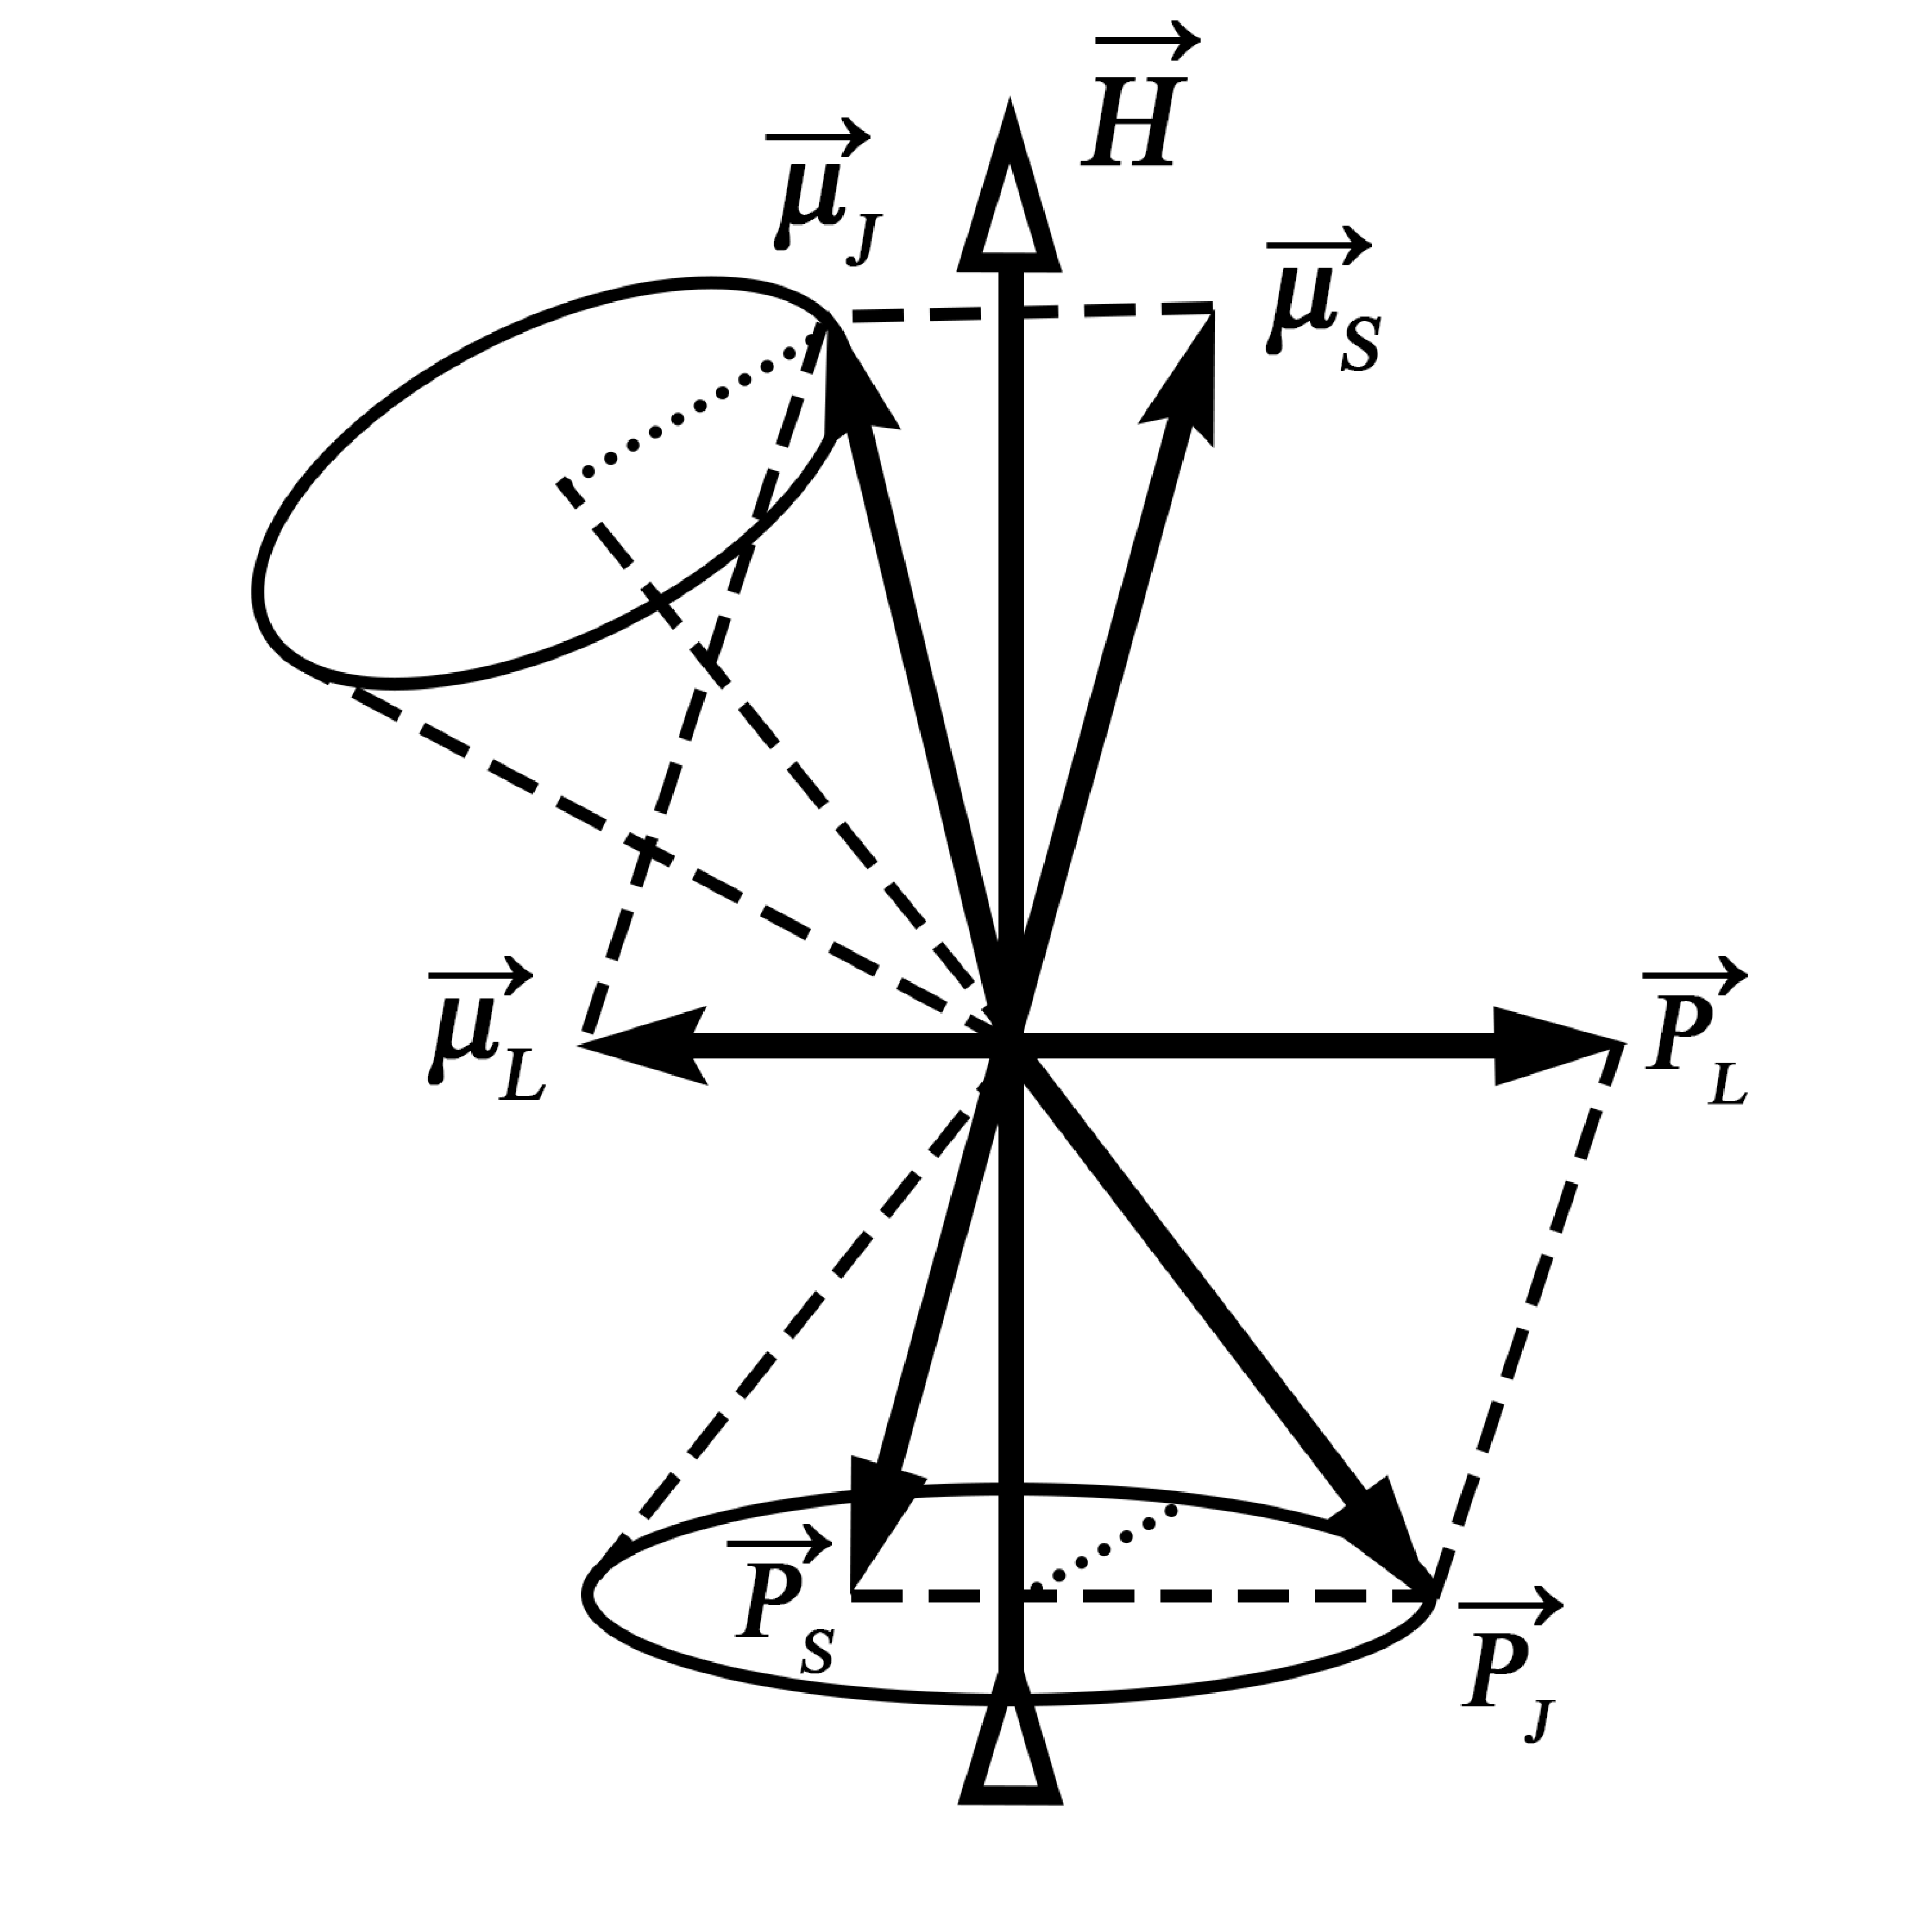
\includegraphics[width=.7\textwidth]{fig/fig2.pdf}
    \caption{Векторная модель атома}    
    \label{fig:2}
\end{figure}


Согласно правилам построения векторной модели складываемые результирующие моменты $\vec{P_L}$ и $\vec{P_S}$ (а вместе с ними и магнитные моменты $\vec{\mu_J}$,$\vec{\mu_L}$,$\vec{\mu_S}$ на векторной диаграмме рис. \ref{fig:2}) прецессируют вокруг направления результирующего момента $\vec{P_J}$. Скорость прецессии пропорциональна величине спин-орбитального взаимодействия.

Качественный вид зеемановского спектра оказывается различным в зависимости от соотношения между величинами взаимодействия результирующих моментов друг с другом и магнитным полем.

Рассмотрим два случая:

1)\textbf{сильное поле} - действие поля на каждый из моментов $\vec{P_L}$ и $\vec{P_S}$ превосходит взаимодействие их между собой

2)\textbf{слабое поле} - взаимодействие моментов друг с другом больше взаимодействия на каждый из них магнитного поля.

\textbf{1)} Внешнее магнитное поле $\vec{H}$ разрывает связь между результирующими моментами $\vec{P_L}$ и $\vec{P_S}$, и каждый из них прецессирует вокруг направления поля независимо другого. Проектироваться на направление поля $\vec{H}$ векторы $\vec{P_L}$ и $\vec{P_S}$ (а значит и векторы $\vec{\mu_L}$ и $\vec{\mu_S}$) будут тоже каждый в отдельности: $\vec{\mu_H}=-\gamma \hbar(M_L+2M_S)$, то есть расщепление оказывается целым кратным $\mu_0 H$. Для переходов имеют место правила отбора: $\Delta M_L=0,\pm 1; \Delta M_S=0.$ В результате получается триплет, совпадающий по виду с {\itshape\textbf{нормальным зеемановским триплетом}}, а само явление называется {\itshape\textbf{эффектом Пашена-Бака}}. Этот эффект наблюдается при $H\geq 2\cdot10^5 \text{э}$, когда магнитное расщепление линий становится больше {\itshape\textbf{мультиплетного}} (связанного со спин-орбитальным взаимодействием) расщепления.

\textbf{2)} В случае {\itshape\textbf{слабого магнитного поля}} (именно этот случай реализуется в условиях нашего эксперимента) магнитный момент атома $\vec{\mu_J}$ прецессирует вокруг направления $\vec{H}$ (вместе с вектором $\vec{P_J}$), как это известно из классической механики, но и вокруг самого вектора $\vec{P_J}$. Поскольку частота {\itshape\textbf{классической (ларморовской)}} прецессии пропорциональна величине $H$, в достаточно слабых полях ларморовскую прецессию можно считать медленной по сравнению с прецессией вокруг $\vec{P_J}$. Усредняя $\vec{\mu_J}$ по периоду "быстрой" прецессии, находим, что средний по времени магнитный момент атома $\vec{\mu}$ совпадает с проекцией $\vec{\mu_J}$ на направление $\vec{P_J}$, то есть равен: 
\begin{gather} 
\label{eq:18} 
\mu=\mu_L \cos(\widehat{\vec{\mu_L},\vec{P_J}})+\mu_S \cos(\widehat{\vec{\mu_S},\vec{P_J}})
\end{gather}

Из элементарной геометрии Согласно рис.\ref{fig:2} следует:
\begin{equation} 
\label{eq:19a} 
\cos(\widehat{\vec{P_L},\vec{P_J}})=\frac{P_J^2+P_L^2-P_S^2}{2P_L P_J},
\end{equation}

\begin{gather} 
\label{eq:19b} 
\cos(\widehat{\vec{P_S},\vec{P_J}})=\frac{P_J^2+P_S^2-P_L^2}{2P_S P_J},
\end{gather}
что позволяет переписать равенство (\ref{eq:18}) в виде:
\begin{gather} 
\label{eq:20} 
\mu=\gamma P_J(1+\frac{P_J^2+P_S^2-P_L^2}{2P_J^2}=\mu_0 \text{g} \frac{P_J}{\hbar}.
\end{gather}
 
 Подстановка формул вида (\ref{eq:6}) в (\ref{eq:20}) позволяет сразу найти связь между механическим $P_J$ м "эффективным" магнитным моментом атома $\mu$ в состоянии с квантовыми числами \textbf{J, L, S}, то есть \textbf{g}-фактор данного квантового состояния.
$$\gamma=\frac{e}{2m_ec}$$
$$\vec{\mu_{L_i}} = -\gamma \vec{P_{L_i}}$$
$$\vec{\mu_{S}} = -2\gamma \vec{P_{S_i}}$$
$$g_l=1, g_s=2$$
$$\vec{\mu}=\vec{\mu_{L}}+\vec{\mu_{S}}=-(g_l\vec{L}+g_s\vec{S})\gamma$$
Усреднение магнитного момента $\widehat{\vec{J}}=\widehat{\vec{L}}+\widehat{\vec{S}}$
$$\widehat{\vec{J^2}}=\widehat{L^2}+\widehat{S^2}+2(\widehat{\vec{L}},\widehat{\vec{S}})$$
$$(\widehat{\vec{L}},\widehat{\vec{S}})=\frac12(\widehat{J^2}-\widehat{L^2}-\widehat{S^2})$$
$$(\widehat{\vec{\mu}},\widehat{\vec{J}})=-\gamma(g_l\vec{L}+g_s\vec{S})(\widehat{\vec{L}}+\widehat{\vec{S}})=-\gamma(g_l{L^2}+g_s{S^2}+(g_l+g_s)(\widehat{\vec{L}},\widehat{\vec{S}}))$$
По аналогии вводится g=фактор для полного магнитного момента
$$(\widehat{\vec{\mu}},\widehat{\vec{J}})=-g\gamma\widehat{\vec{J^2}}, \vec{\mu_J}=-g_J\gamma\widehat{\vec{J}} $$
$$-g\gamma\widehat{\vec{J^2}}=-\gamma(g_l{L^2}+g_s{S^2}+(g_l+g_s)\frac12(\widehat{J^2}-\widehat{L^2}-\widehat{S^2}))$$
$$g=\frac{1}{\widehat{J^2}}(_l{L^2}+g_s{S^2}+\frac12g_l\widehat{J^2}-\frac12g_l\widehat{L^2}-\frac12g_l\widehat{S^2}+\frac12g_s\widehat{J^2}-\frac12g_s\widehat{L^2}-\frac12g_s\widehat{S^2})$$
\begin{gather} 
\label{eq:21} 
\text{g}=1+\frac{J(J+1)+S(S+1)-L(L+1)}{2J(J+1)}
\end{gather}
\subsection{Интенсивность зеемановских линий}
%!TEX root = ../zeeman.tex

Реально наблюдаемое в эксперименте число зеемановских линий существенным образом зависит от их относительных интенсивностей. Интенсивности зеемановских компонент могут быть рассчитаны из соображений симметрии. Результаты расчетов приведены в \ref{tab:1}.

В качестве примера приведем результаты расчета зеемановского спектра, соответствующего переходу 
$J\rightarrow J+1$
 между комбинирующими уровнями 
 $E_1(J_1=1,L_1=2,S_1=1)$ и $E_2(J_2=2,L_2=2,S_2=1)$,
  тогда согласно формуле \ref{eq:21} 
  $g_1=\frac12$, $g_2=\frac32$. 
  Переходы, на которых возможно получение зеемановских компонент, показаны стрелками на рис.\ref{fig:3}, а в таблице \ref{tab:2} приведены поляризация и интенсивности соответствующих линий. 

 Как видно из \ref{eq:11} и таблиц \ref{tab:1}, \ref{tab:2}, зеемановский спектр зеркально симметричен относительно несмещенной линии, поэтому достаточно рассчитать половину спектра.

 \renewcommand{\arraystretch}{2}
\begin{table}[H]
    \caption{Относительные интенсивности зеемановских компонент}
    \centering
    %\resizebox{\textwidth}{!}{%
    \begin{tabular}{|c|c|c|c|c|}
    \hline
    \textbf{Переход} & $J\rightarrow J-1$ &$J\rightarrow J$ & $J\rightarrow J+1$ \\ \hline
    \end{tabular}%
    \label{tab:1}
    % }
\end{table} 

\begin{table}[H]
    \setlength{\tabcolsep}{8pt}
    \caption*{Поперечный эффект}
    \centering 
    \begin{tabular}{|c|c|c|c|c|}
    \hline
    $M \rightarrow M-1$ & $ \frac{(J+M-1)(J+M)}{4} $ & $\frac{(J-M+1)(J+M)}{4}$ & $\frac{(J-M+2)(J-M+1)}{4}$ \\ \hline
    $M \rightarrow M$ & $ (J+M)(J-M) $ & $M^2$ & $(J+M+1)(J-M+1)$ \\ \hline
    $M \rightarrow M+1$ & $ \frac{(J-M-1)(J-M)}{4} $ & $\frac{(J+M+1)(J-M)}{4}$ & $\frac{(J+M+2)(J+M+1)}{4}$ \\ \hline
    \end{tabular}
\end{table}

\begin{table}[H]
    \setlength{\tabcolsep}{8pt}
    \caption*{Продольный эффект}
    \centering 
    \begin{tabular}{|c|c|c|c|c|}
    \hline
    $M \rightarrow M-1$ & $ \frac{(J+M-1)(J+M)}{2} $ & $\frac{(J-M+1)(J+M)}{2}$ & $\frac{(J-M+2)(J-M+1)}{2}$ \\ \hline
    $M \rightarrow M+1$ & $ \frac{(J-M-1)(J-M)}{2} $ & $\frac{(J+M+1)(J-M)}{2}$ & $\frac{(J+M+2)(J+M+1)}{2}$ \\ \hline
    \end{tabular}
\end{table}

\begin{figure}[H]
    \centering
    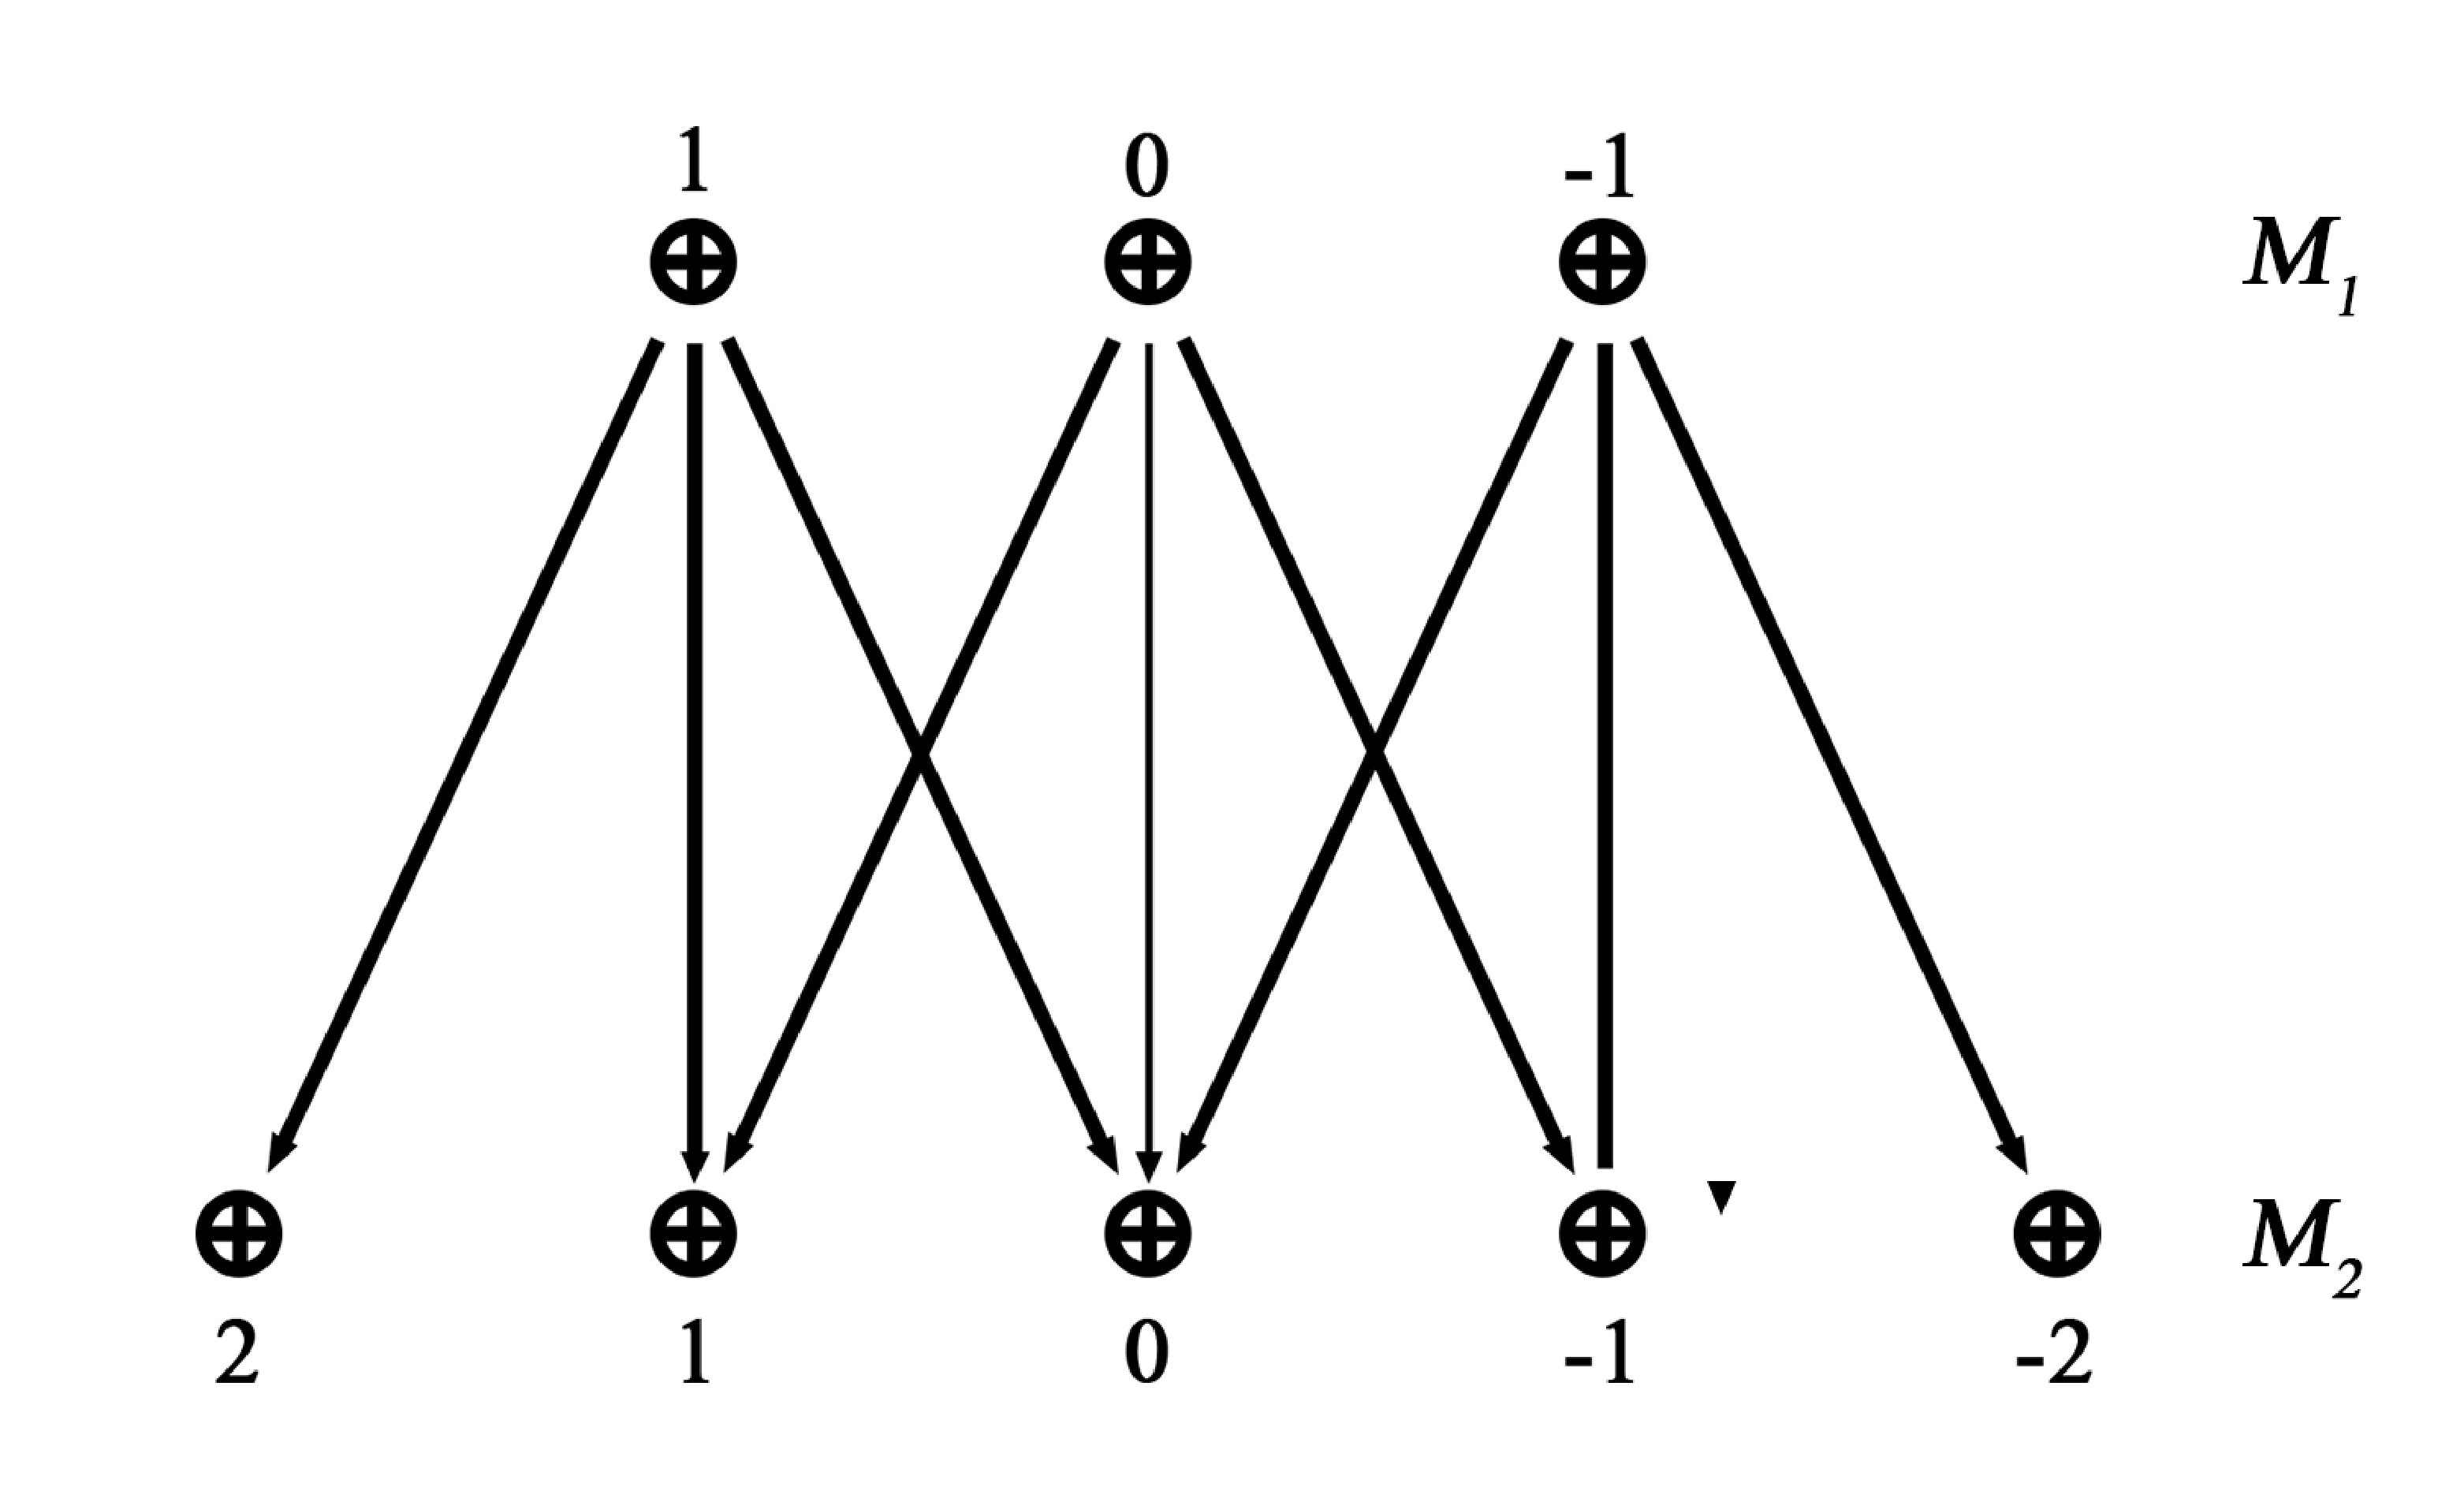
\includegraphics[width=.7\textwidth]{fig/fig3.pdf}
    \caption{Пример излучательных переходов, разрешенных правилами отбора} 
    \label{fig:3}   
\end{figure}


\begin{table}[H]
    \setlength{\tabcolsep}{6pt}
    \caption{Поляризация и интенсивности линий Зеемановского спектра соответствующего переходу $J \rightarrow J+1$ между комбинирующими уровнями $ E_1(J_1=1,L_1=2,S_1=1)$ и $E_2(J_2=2,L_2=1,S_2=1) $} 
    \centering 
    \begin{tabular}{|p{8cm}|c|c|c|c|c|}
    \hline
    $\Delta \omega_{M_1 , M_2} * \hbar / (\mu_0 H) $ & \textbf{0} & $\mathbf{\pm 1/2}$ & $\mathbf{\pm 1}$ & $\mathbf{\pm 3/2}$ & $\mathbf{\pm 5/2}$ \\ \hline
    \textbf{Поляризация}  & $\mathbf{\boldsymbol\pi}$ & $ \mathbf{\boldsymbol\sigma} $ & $\mathbf{\boldsymbol\pi}$ & $ \mathbf{\boldsymbol\sigma} $ & $\mathbf{\boldsymbol\sigma} $ \\ \hline
    \textbf{Интенсивность}  (относительные единицы, поперечный эффект) & \textbf{4} &  \textbf{1/2} & \textbf{3}  & \textbf{3/2} & \textbf{3} \\ \hline
    \end{tabular}
    \label{tab:2}
\end{table}

\subsection{Классическая модель Зеемана}
%!TEX root = ../zeeman.tex

Некоторые закономерности эффекта Зеемана могут быть проиллюстрированы на классической модели, которая основывается на том, что движущийся вокруг ядра атома электрон обладает механическим и магнитным моментам связанными соотношением $\vec{\mu}_{l_i}=-\gamma \vec{P}_{l_i}$. Таким образом, классическая модель, в отличие от квантовой, не учитывает собственный механический момент (спин) и магнитный момент электрона и, следовательно, может дать верные результаты лишь в частном случае, когда спины электронов в атоме скомпенсированы ($s=0$). По чисто историческим причинам этот случай получил название \textbf{нормального} (или \textbf{простого}) \textbf{эффекта Зеемана}, тогда как при \textbf{$s\ne0$} эффект Зеемана называют \textbf{аномальным} (или \textbf{сложным}). 

\begin{wrapfigure}{h}{0.4\textwidth}
\begin{center}
\vspace{-50pt}
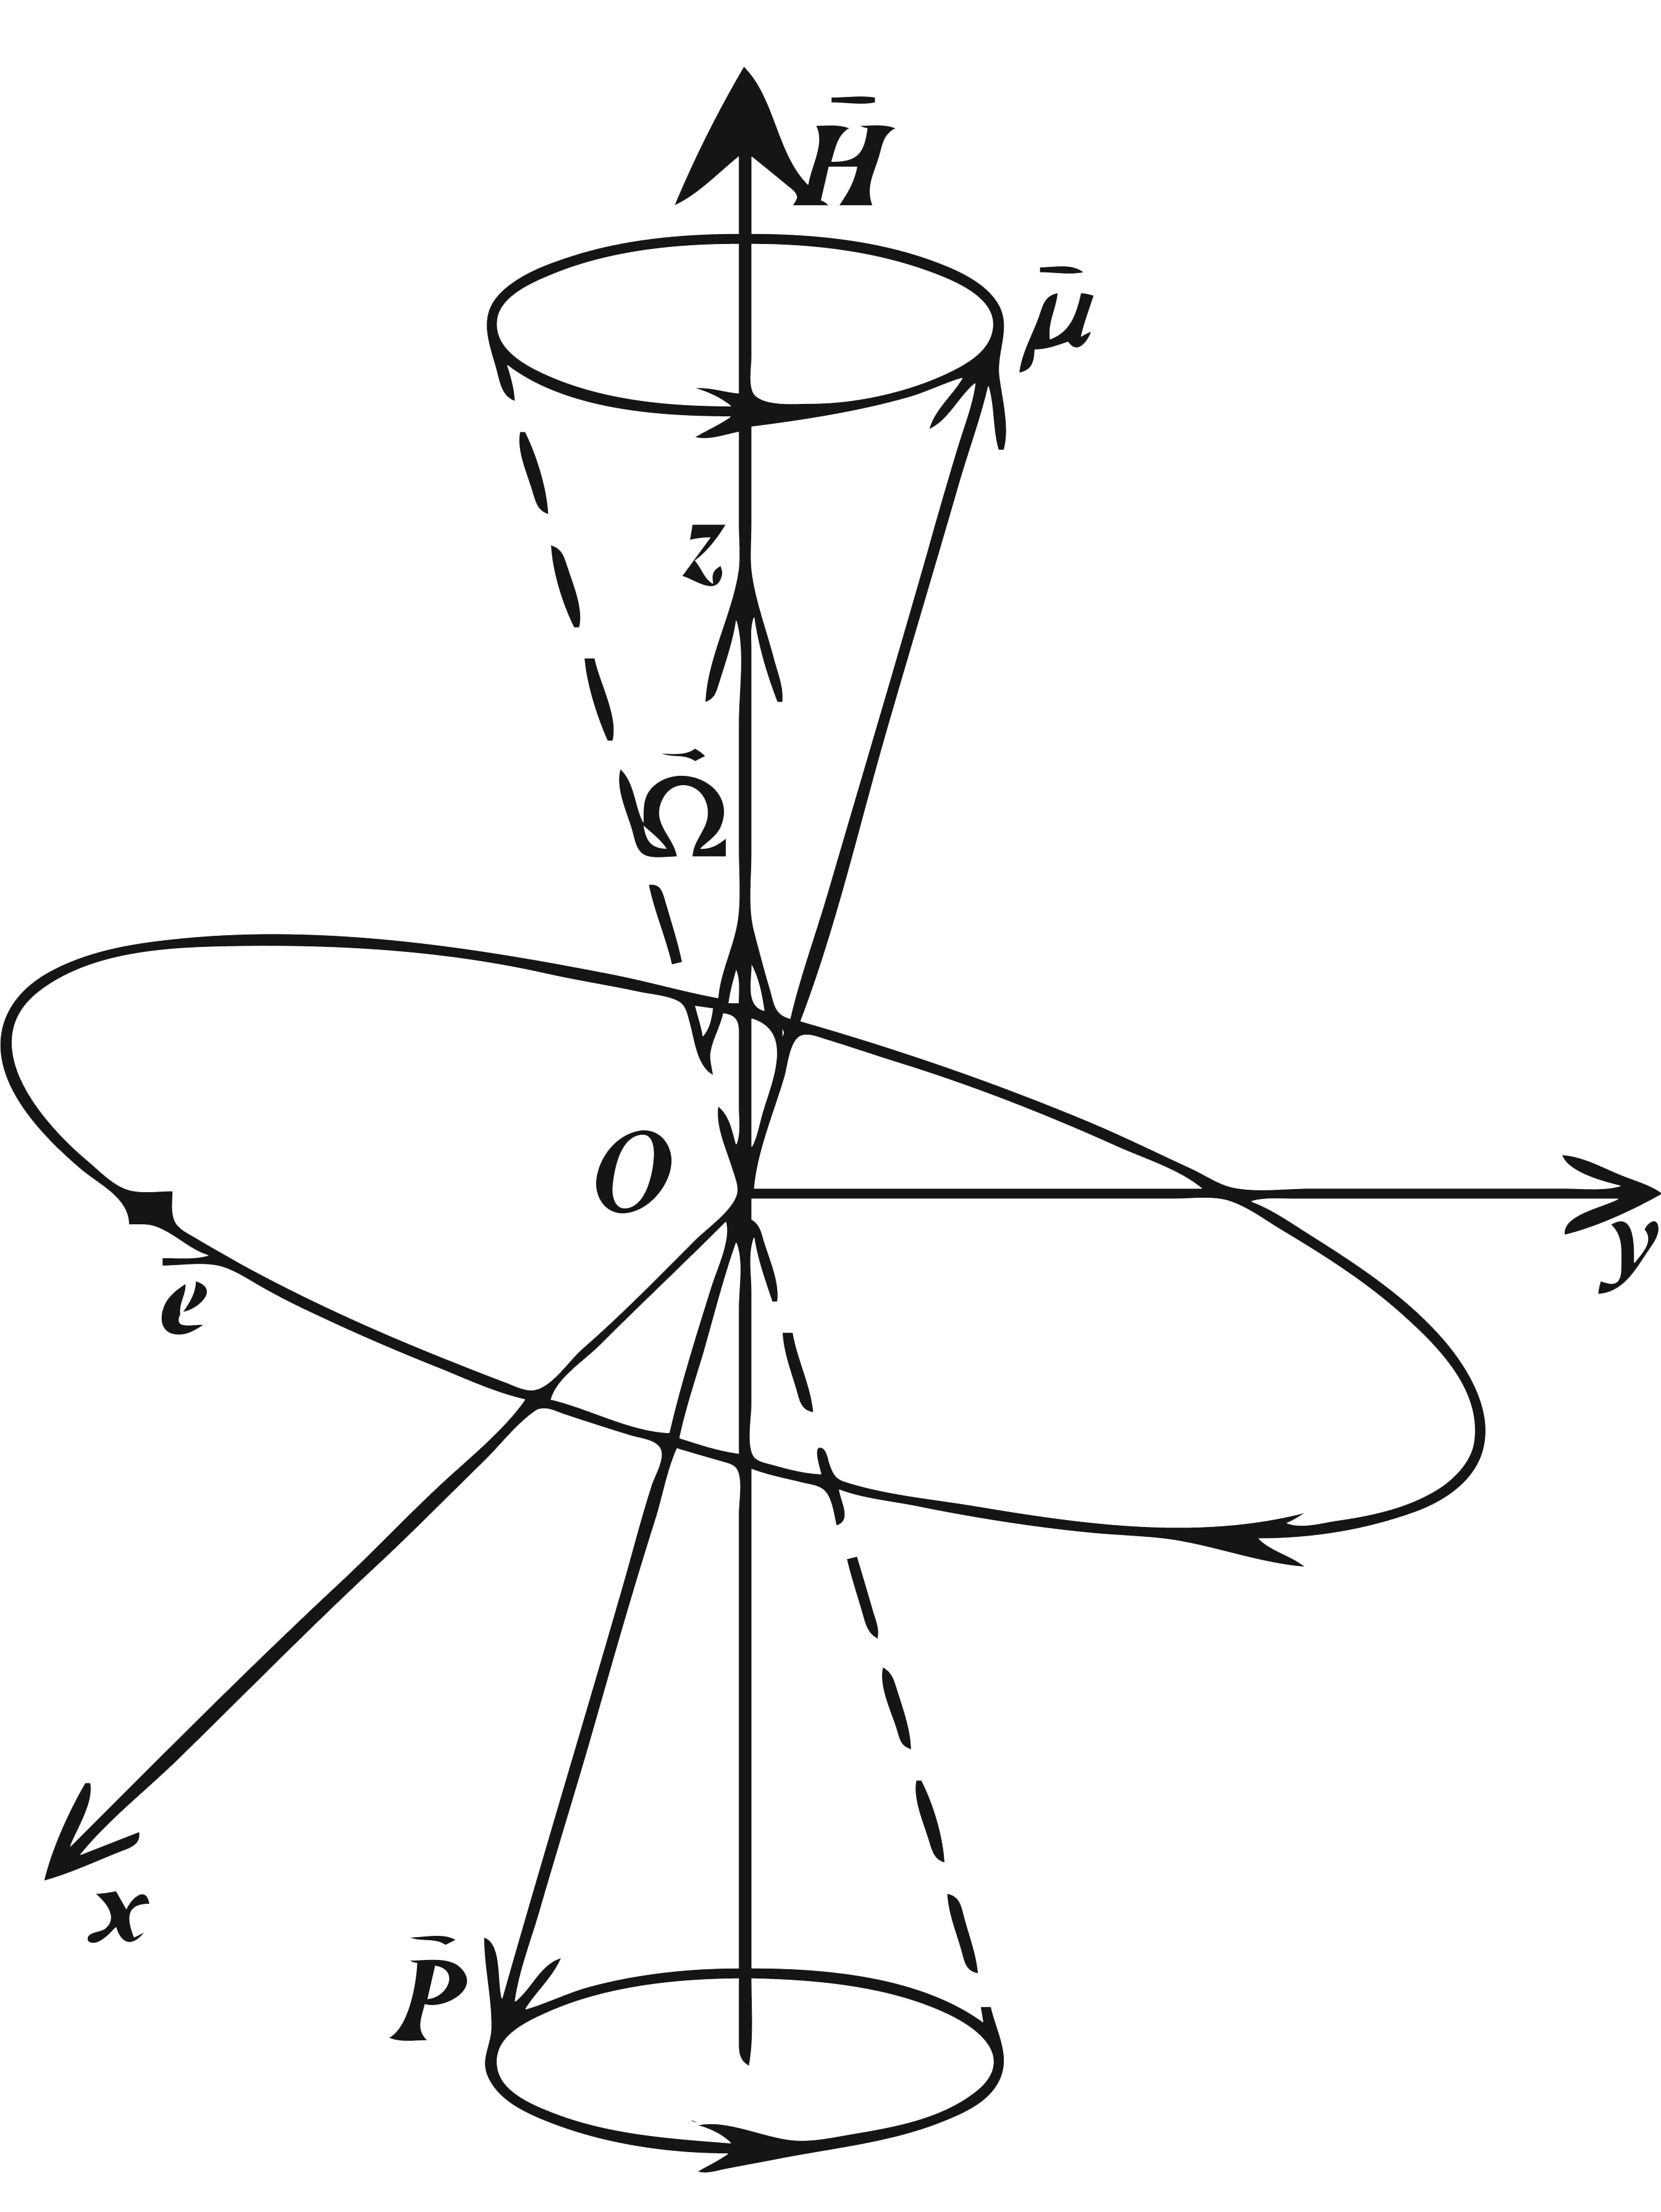
\includegraphics[width=0.4\textwidth]{fig/fig4.jpg}
\vspace{-45pt}
\end{center}
\caption{Прецессия электрона в магнитном поле классической модели атома}
\label{fig:4}
\end{wrapfigure}

Как легко показать из законов классической физики, орбитальный электронный ток (т.е. магнитный волчок) во внешнем магнитном поле прецессирует вокруг направления $\vec{H}$ с ларморовской частотой: 
\begin{equation}
	\Omega=\gamma H=\frac{eH}{2mc}.
\end{equation} 
Чтобы объяснить спектральный состав, а также поляризацию нормальных зeемановских компонент, надо разложить сложное движение электрона на более простые составляющие.

Введем лабораторную систему отсчета ($x, y, z$) как показано на \ref{fig:4}магнитное поле $\vec{H}$ направлено по оси $z$, а плоскость ($x, y$)- перпендикулярна ему. 

Пусть сначала магнитное поле отсутствует, то есть $\Omega = 0$ - прецессионного движения нет. Орбитальное движение разложим на движение в плоскости ($x, y$) и вдоль оси $z$. Проекция кругового орбитального движения на плоскость ($x, y$) является движением по эллипсу, которое, в свою очередь, можно представить в виде суммы двух круговых вращений, как это показано на \ref{fig:5}. 

% \begin{wrapfigure}{h}{0.6\textwidth}
% \begin{center}
% \vspace{-10pt}
% 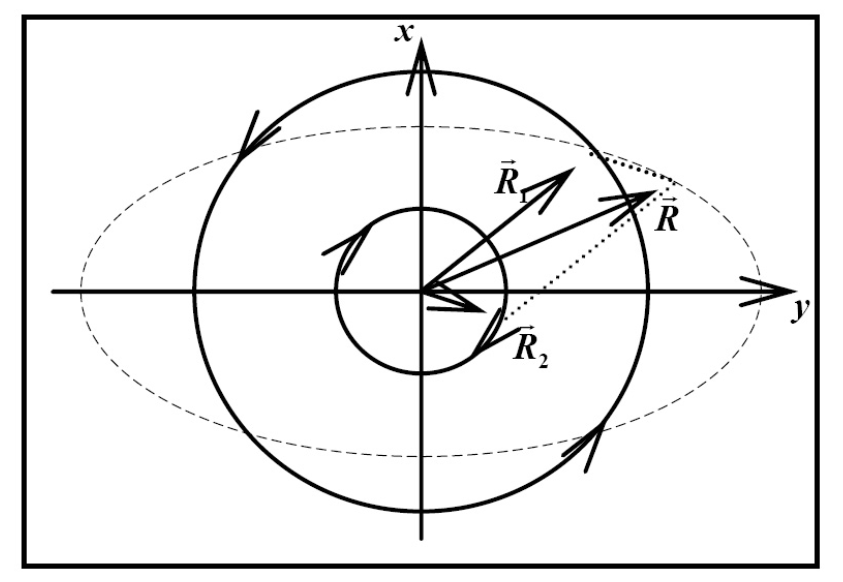
\includegraphics[width=0.6\textwidth]{fig/fig5.jpg}
% \vspace{-35pt}
% \end{center}
% \caption{Диаграмма, иллюстрирующая представление движения по эллипсу в виде суммы двух круговых}
% \label{fig:5}
% \end{wrapfigure}

\begin{figure}[tb]
	\centering
	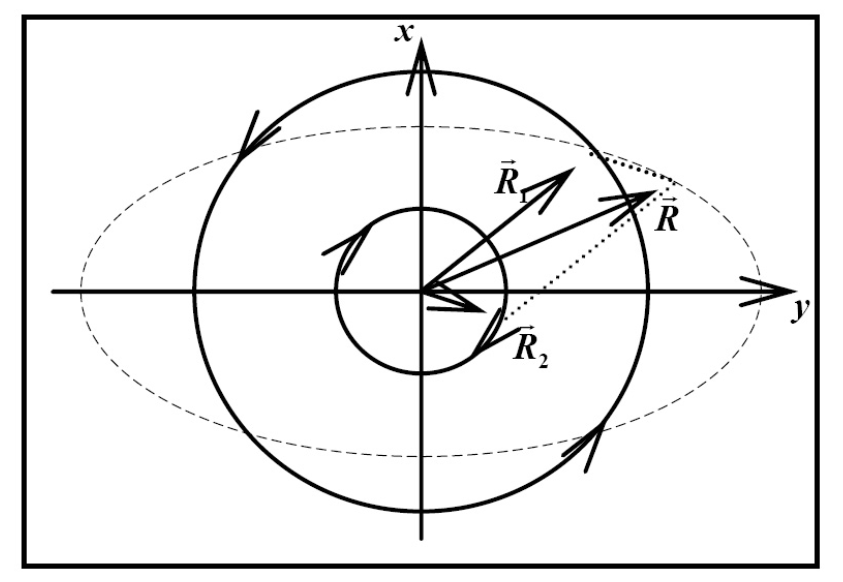
\includegraphics[width=0.6\textwidth]{fig/fig5.jpg}
	\caption{Диаграмма, иллюстрирующая представление движения по эллипсу в виде суммы двух круговых}
	\label{fig:5}
\end{figure}

Здесь вектора $\vec{R}_1$ и $\vec{R}_2$ вращаются в противоположных направлениях с угловой скоростью орбитального движения $\omega_0$ симметрично относительно большой оси эллипса, при этом конец вектора $\vec{R}$ двигается по эллипсу, большая полуось которого равна $|\vec{R}_1 + \vec{R}_2|$, а малая $|\vec{R}_1 - \vec{R}_2|$.

В свою очередь, разложив круговое орбитальное движение электрона на сумму двух линейных ортогональных гармонических колебаний, легко увидеть, что проекция этого движения на ось $z$ есть гармоническое колебание c частотой $\omega_0$.

При включении магнитного поля, как уже отмечалось выше, результирующее движение электрона будет суммой быстрого орбитального вращения и прецессии орбиты, то есть на орбитальное движение наложится вращение с угловой скоростью $\Omega$ вокруг оси $z$. Колебания вдоль оси $z$ при этом не изменятся, скорость вращения вектора $\vec{R}_1$ уменьшится, а вектора $\vec{R}_2$ увеличится на величину $\Omega$. 

Используя элементарную дипольную модель излучающего атома, легко увидеть что в спектре излучения вдоль направления внешнего магнитного поля будут присутствовать лишь две циркулярно поляризованные волны с частотами $\omega_{1,2}=\omega \pm \Omega$ (\textbf{нормальный зеeмановский дублет}), тогда как в перпендикулярном направлении будут наблюдаться три линейно поляризованные компоненты на частотах $\omega_1, \omega_0, \omega_2$ (\textbf{нормальный зеeмановский триплет}).

Поскольку расщепление линии обычно весьма мало, т.е. $|\omega_1 - \omega_2|\ll \omega_0$, из статистических соображений следует, что средняя кинетическая энергия каждой из трех составляющих движения (степеней свободы) электрона примерно одинакова. Это означает, что, если в отсутствие магнитного поля интенсивность линии излучения обозначить $I_0$, то интенсивности зеeмановских компонент составят $I_0/2$ и $I_0/2$ в дублете и $I_0/4, I_0/2, I_0/4$ в триплете. 

Таким образом, классическая теория предсказывает сам факт расщепления спектральных линий в магнитном поле, хорошо объясняет поляризацию излучения и качественно указывает на различную относительную интенсивность зеемановских компонент.
Число наблюдаемых зеемановских линий, их частоты и относительные интенсивности должны рассчитываться по приведенным выше квантомеханическим формулам.


% %%%%%%%%%%%%%%%%%%%%%%%%%%%%%%%%%%%%%%%%%%%%%%%%%%%%%%%%%%%%%%%%%%%%%%%%
>>>>>>> практика
\section{Практическая часть}
%!TEX root = ../zeeman.tex
\begin{figure}[H]{}
\centering
\vspace{-10pt}
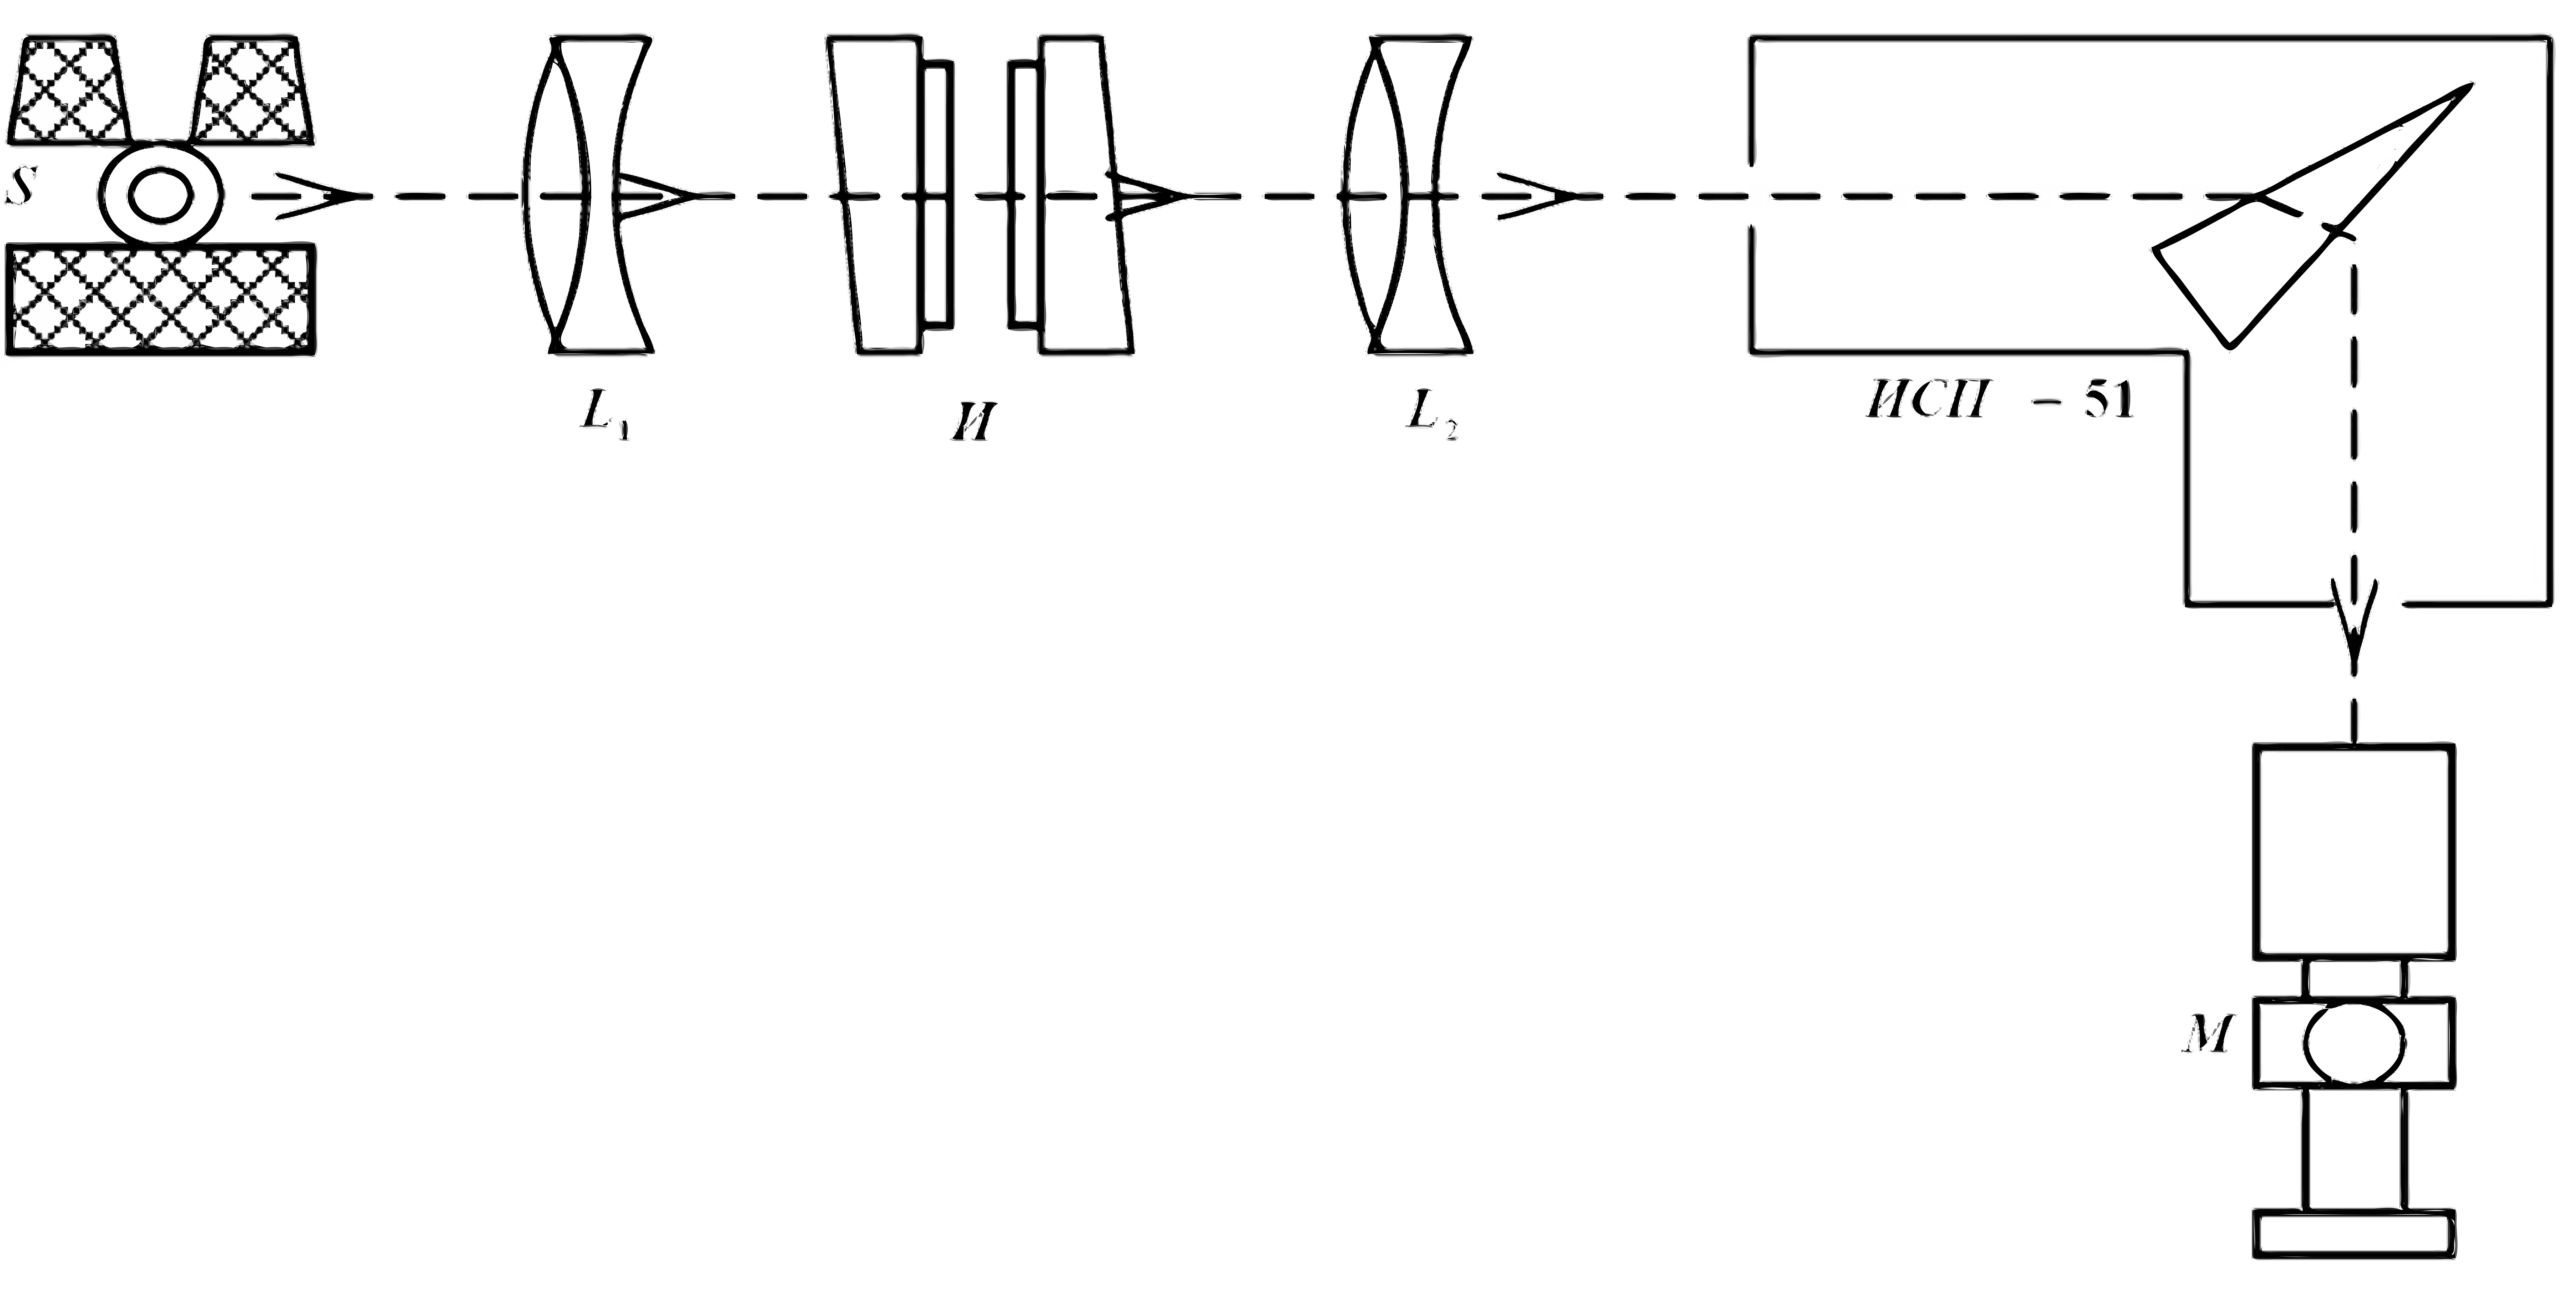
\includegraphics[width=0.9\textwidth]{fig/fig6.jpg}
\vspace{-40pt}

\caption{Cхема экспериментальной установки} \label{fig:6}
\end{figure}

Целью данной работы является изучение эффекта Зеемана на примере спектра излучения $Ne$ с помощью \textbf{интерферометра Фабри-Перо (ИФП)}.

Схема экспериментальной установки приведена на \ref{fig:6}. Здесь $S$ - газосветная трубка, помещенная между полюсами поворачивающегося электромагнита, \textbf{И-ИФП}, $L_1$ и $L_2$ - ахроматические линзы, \textbf{ИСП-51} - призменный спектрограф, \textbf{T} - короткофокусная зрительная трубка, \textbf{M} - окулярный микрометр. 

\textbf{ИФП} является многолучевым интерферометром высокой разрешающей способности. Он состоит из двух прозрачных клиновидных пластин (см. рис. \ref{fig:7}), внутренние поверхности которых ограничивают плоскопараллельный слой воздуха. На эти поверхности нанесено диэлектрическое покрытие, обеспечивающие энергетический коэффициент отражения $\rho$, близкий к единице. 

\begin{wrapfigure}{h}{0.4\textwidth}

\begin{center}
\vspace{-25pt}
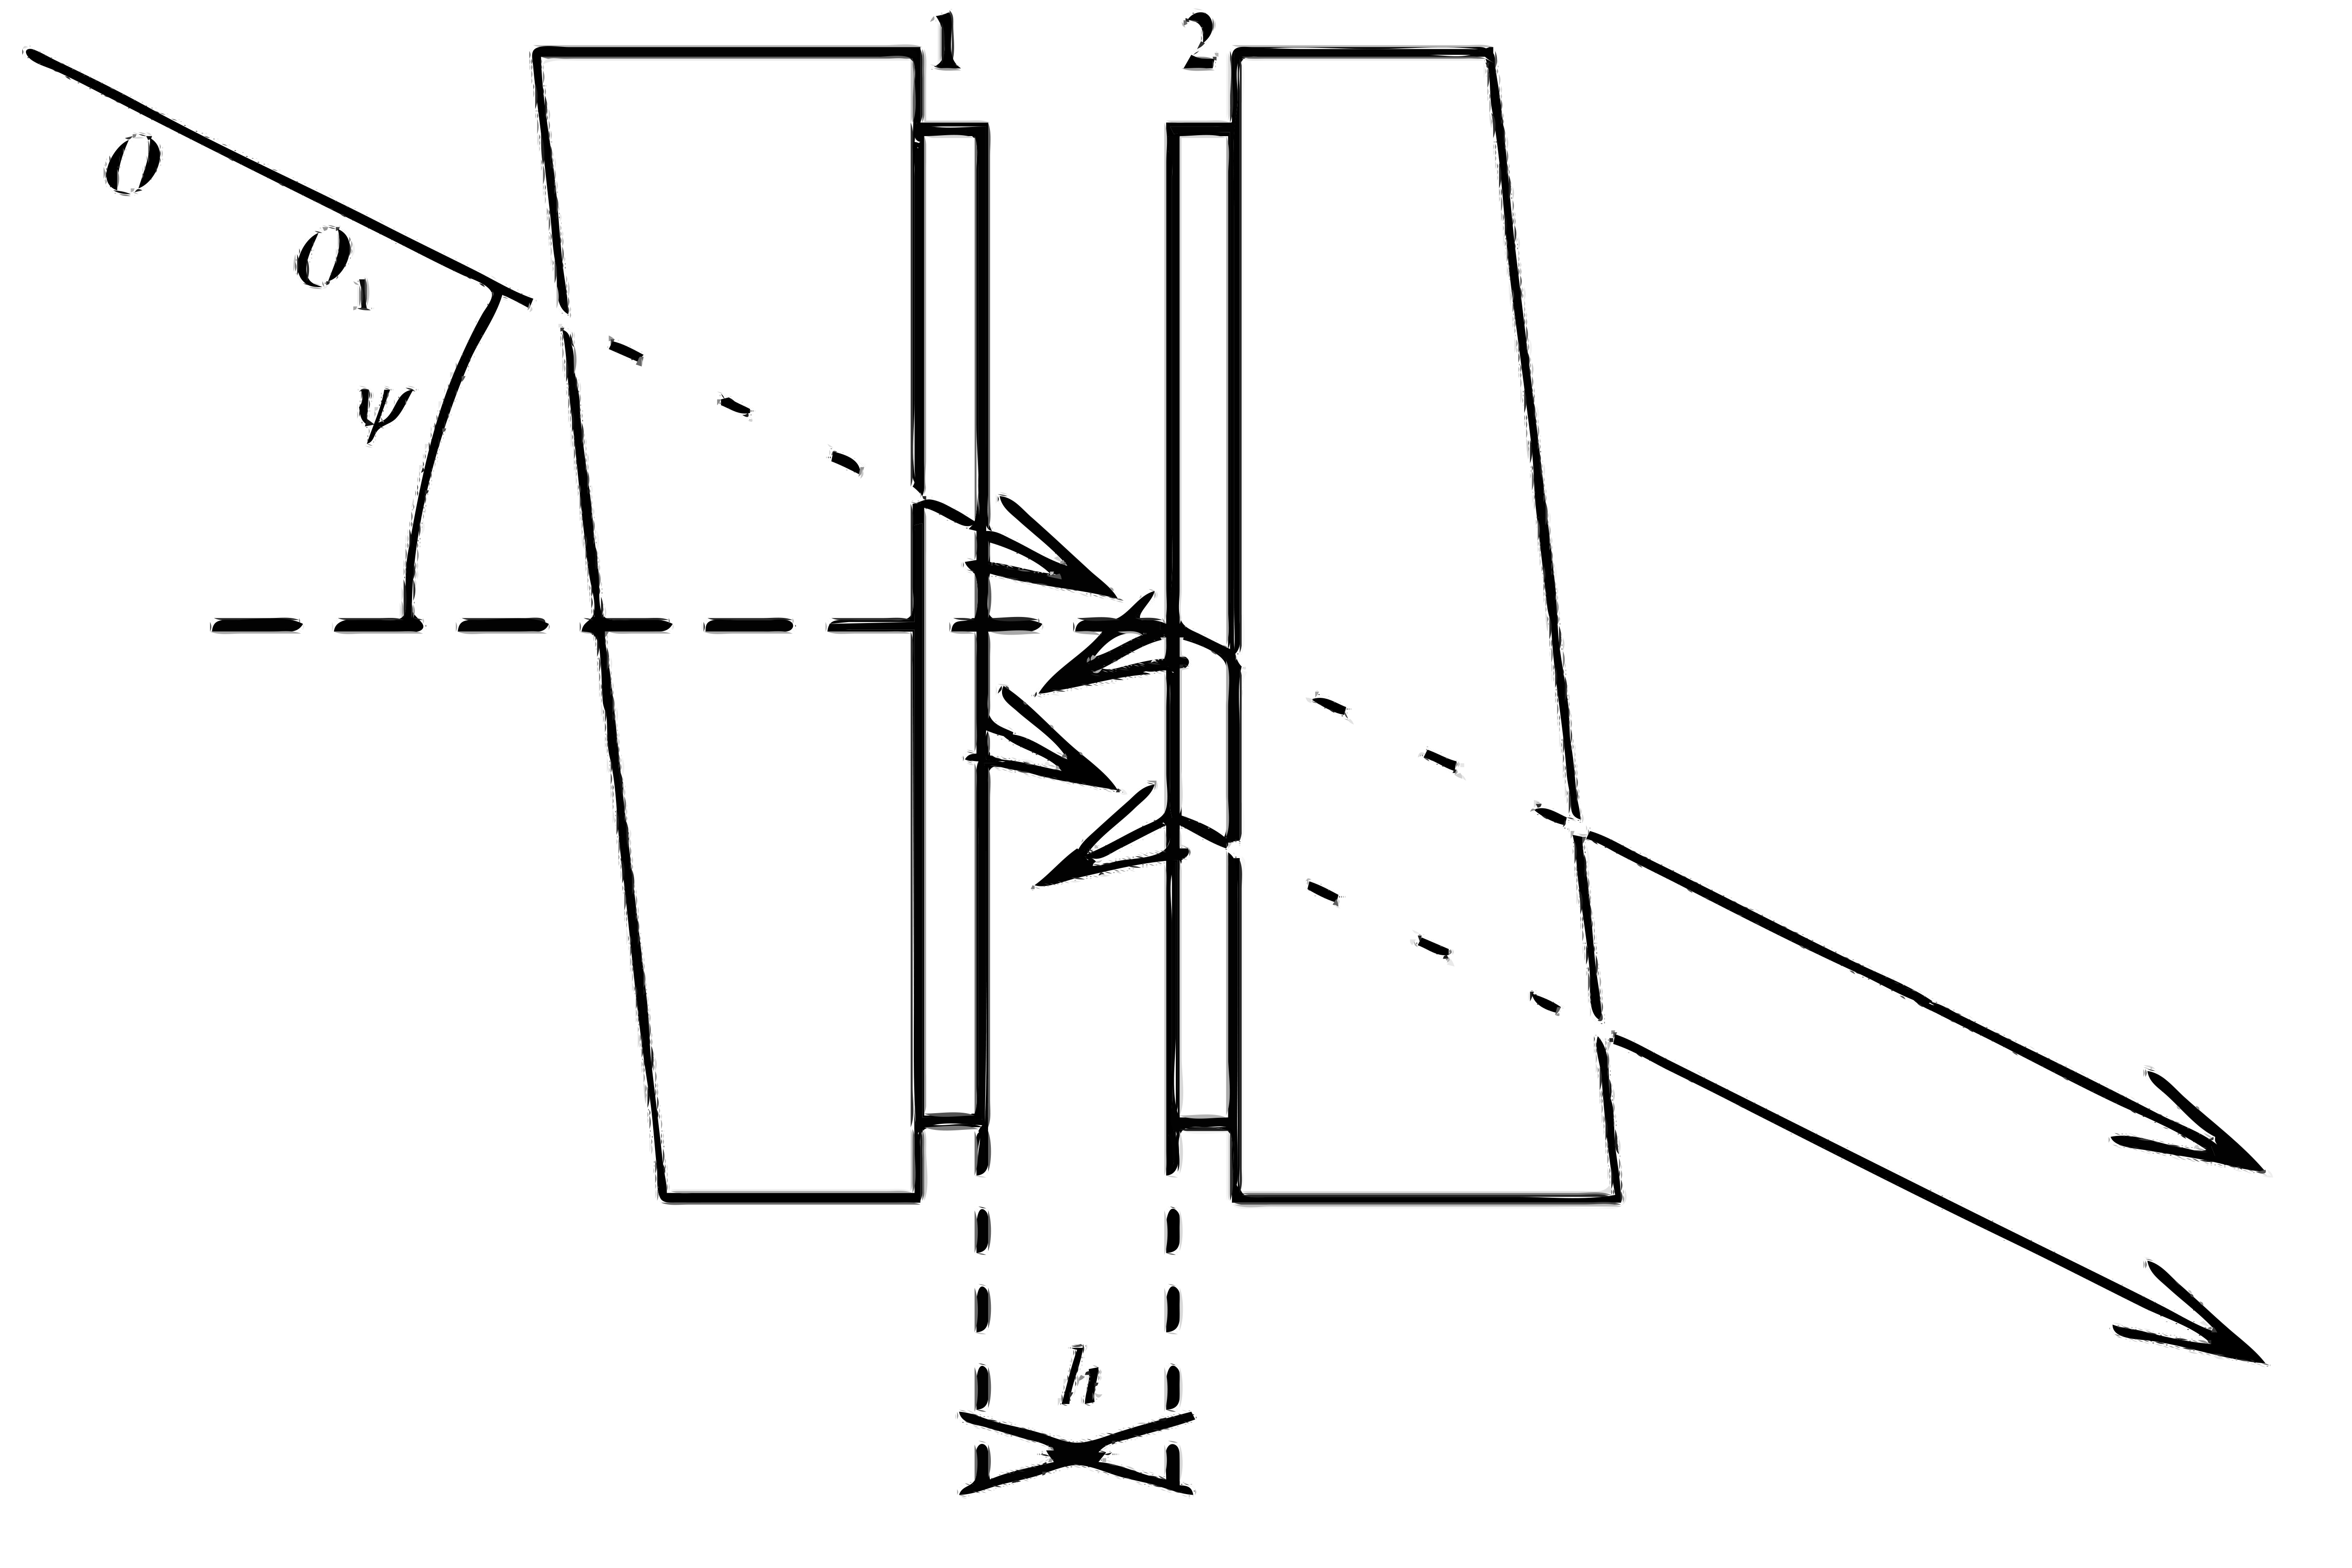
\includegraphics[width=0.4\textwidth]{fig/fig7.jpg}
\caption{Интерферометр Фабри-Перо} \label{fig:7}
% \vspace{-40pt}

\end{center}

\end{wrapfigure}

Луч $OO_1$, вошедший в интерферометр и многократно отразившийся от зеркальных поверхностей 1 и 2, образует ряд проходящих параллельно лучей с постоянной разностью хода 
\begin{equation}
	\Delta=2h \cos \Psi,
\end{equation} где $h$ толщина воздушного слоя, $\Psi\ll 1$-- угол падения света в зазоре. 

Объектив, установленный за \textbf{ИФП}, формирует \textbf{линии равного наклона}, представляющие собой систему концентрических колец. Угловые радиусы $\Psi_1$ колец Фабри-Перо для длины волны $\lambda$ удовлетворяют условию интерференционных максимумов 
\begin{equation}
\label{eq:24}
	2h \cos \Psi_i = m_i \lambda=m_0 \lambda \cos \Psi_i,
\end{equation}

где $m_i$ - порядок интерференции (большое целое число, так как $h \gg \lambda$); $m_0=2h/\lambda$ - максимальный порядок интерференции, получающийся при $\Psi=0$, то есть в центре картины; $i=1, 2, 3,\dots$ - номер кольца по порядку от центра картины. 



Легко показать, что диаметры колец Фабри-Перо описываются формулой: 
\begin{equation}
	\label{eqL25}
	d_i^2=\frac{4 f^2 \lambda (i-1+\varepsilon_{\lambda})}{h}
\end{equation}
где $f$ - фокусное расстояние объектива $\varepsilon_{\lambda} \in [0;1]$ - так называемая дробная доля порядка интерференции в центре колец, определяемая равенством 
\begin{equation}
	\label{eq:26}
	m_0 - m_i=i-1+\varepsilon_{\lambda}.
\end{equation}

 Характерными особенностями \textbf{ИФП} как спектрального прибора являются высокая \textbf{разрешающая способность}
 \begin{equation}
 	\label{eq:27}
 	R=\frac{m_i \pi \sqrt{\rho}}{1-\rho}
 \end{equation}
 
и малая \textbf{дисперсионная область}
\begin{equation}
	\label{eq:28}
 	\Delta \lambda_{\text{своб}}=\frac{\lambda^2}{2h \cos \Psi}.
 \end{equation} 

Как правило, это делает необходимым использование дополнительного \textbf{монохроматора}. В нашем случае им служит \textbf{призменный спектрограф ИСП-51}.
\begin{figure}[H]
	\begin{center}
	% \vspace{}
	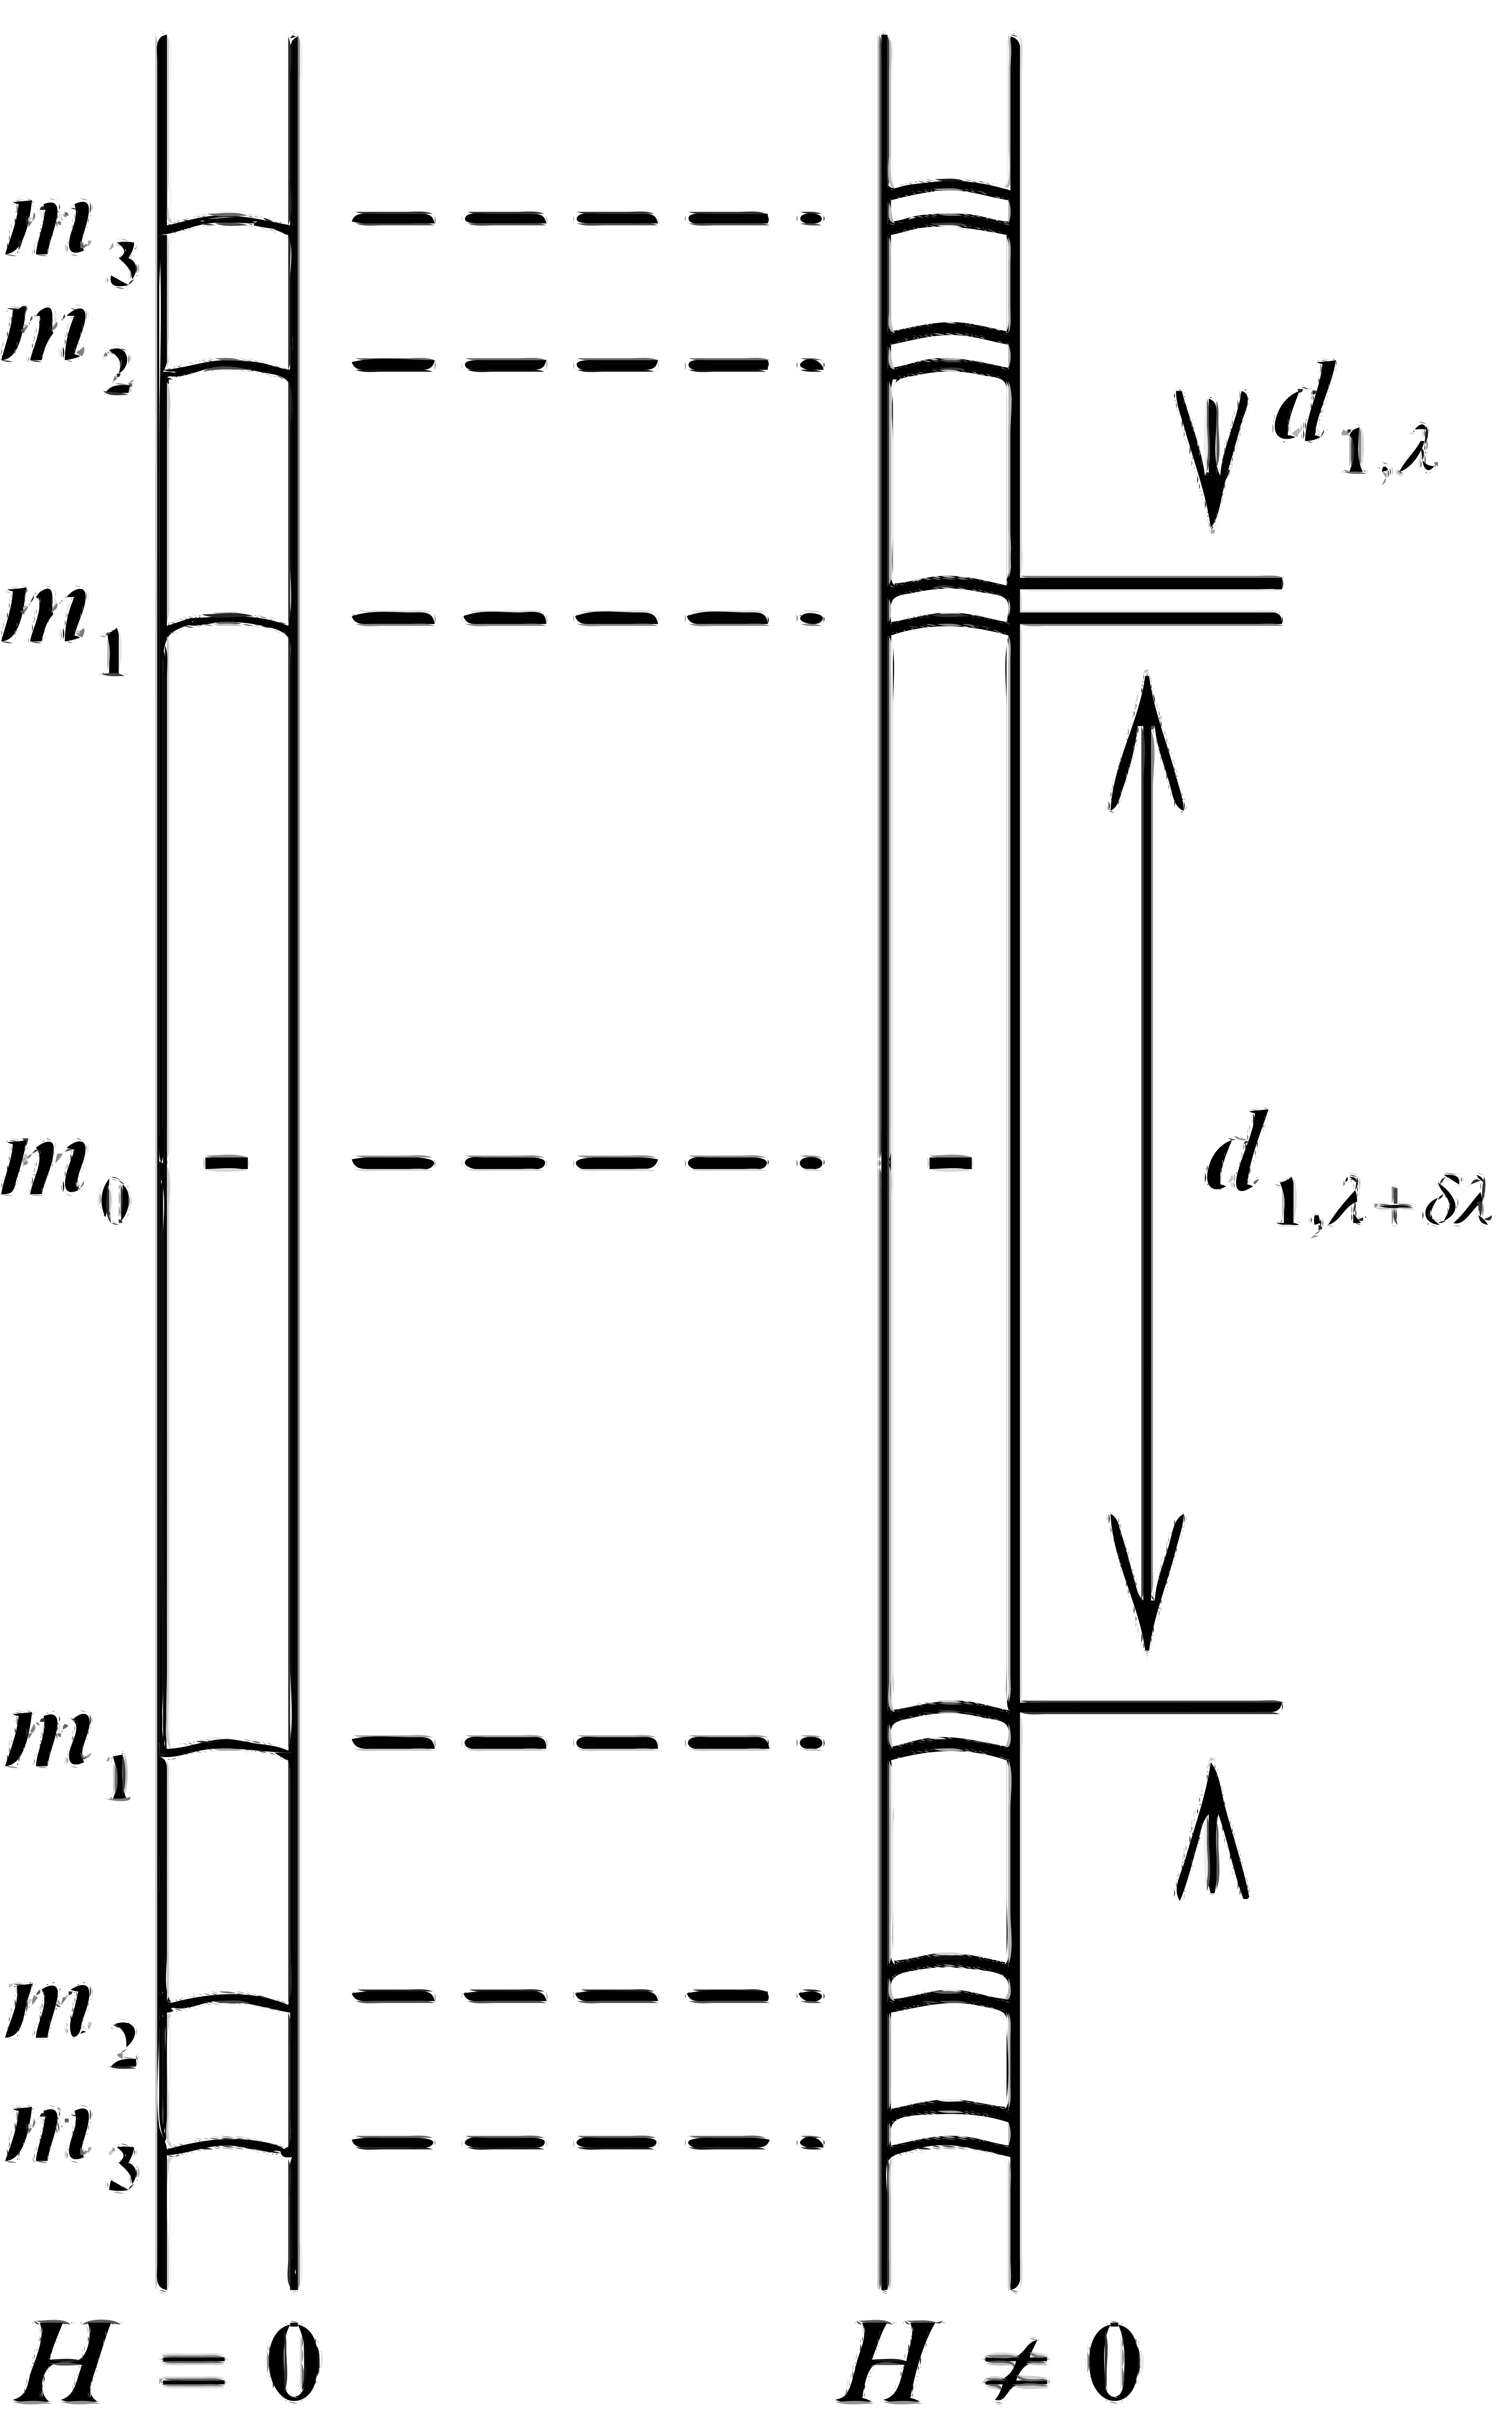
\includegraphics[width=0.4\textwidth]{fig/fig8.jpg}
	% \vspace{-10pt}
	\caption{Вид спектральных линий в выходной плоскости спектрографа}\label{fig:8}
\end{center}

\end{figure}
ИФП устанавливается таким образом, чтобы плоскость локализации колец Фабри-Перо совместилась с плоскостью входной щели спектрографа. Щель вырезает из колец узкую вертикальную полоску. Таким образом, спектрограф разлагает свет в горизонтальной плоскости, а ИПФ - вдоль вертикальной входной щели спектрографа. В результате наблюдения картина, состоящая из ряда светлых вертикальных полосок, прорезанных яркими дугами колец Фабри-Перо. Положение колец определяет тонкую структуру соответствующей спектральной линии. 

Параллельные пучки лучей, вышедших из интерферометра Фабри-Перо (\ref{fig:7}) в фокальной плоскости объектива образуют систему концентрических колец -- линии равного наклона. Однако в окуляр зрительной трубы видны лишь небольшие участки дуг этих колец, соответствующие различным спектральным линиям неона. Для определения величины расщепления $\delta\lambda$ проводят измерения либо диаметров колец, либо лишь разностей их радиусов. В последнем случае установку надо настроить так, чтобы наблюдались лишь верхние (либо нижние) части колец. При этом можно сделать увеличение трубы больше, что облегчает измерение дуг $x_{\lambda-\Delta \lambda},x_{\lambda},x_{\lambda+\Delta \lambda}$ (см. рис. \ref{fig:9}) и уменьшает ошибки измерений.

Получим формулу для расчёта величины $\delta \lambda$. Условие наблюдения интерференционных колец выражается формулой (\ref{eq:24}). Из рис. \ref{fig:10}  с учётом малости угла $\Psi$ для радиуса кольца $R$ найдем
\begin{equation}
	\label{eq:29}
	R\approx f\Psi,
\end{equation}
где $f$-- фокусное расстояние объектива.


Для разностей радиусов \ref{fig:9} из соотношения \ref{eq:29} получим 
\begin{gather}
	\label{eq:30}
	\Delta R_m \approx f \delta \Psi_m \text{ и } \Delta R_{\lambda} \approx f \delta \Psi_{\lambda} 
\end{gather}
%рис 9
\begin{figure}[H]
	\centering
	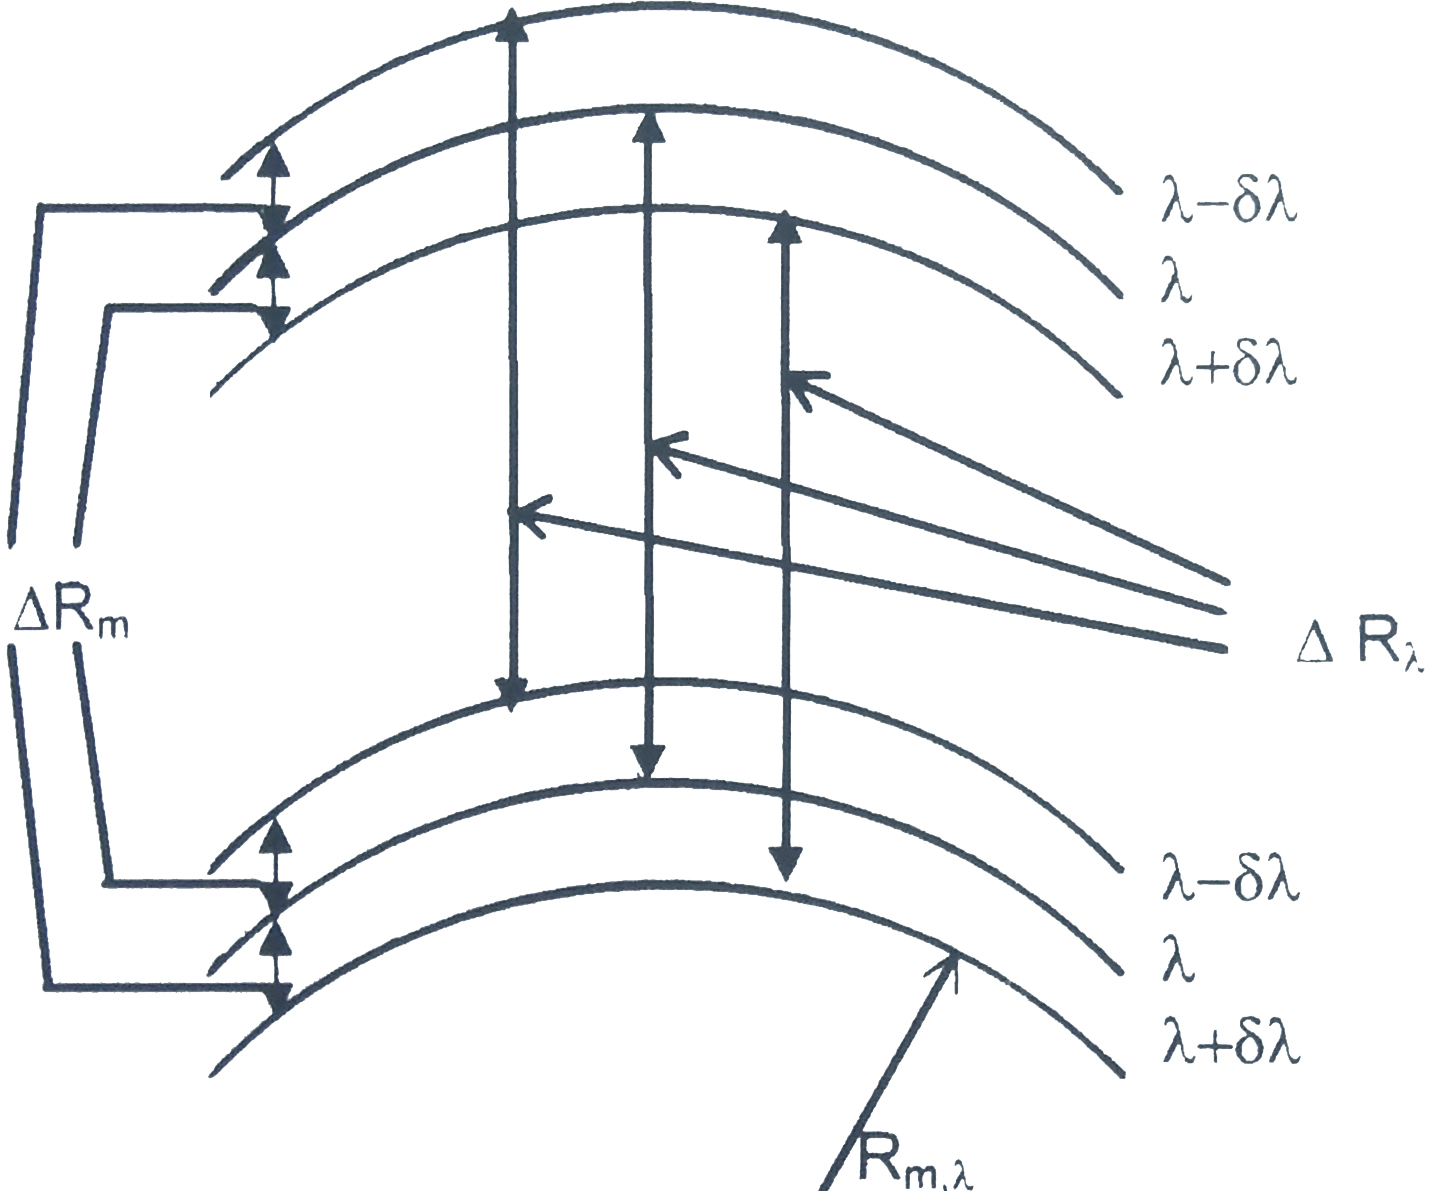
\includegraphics[width=0.7\linewidth]{fig/fig9.jpg}
	\caption{Вид двух соседних колец интерферометра Фари-Перо при расщеплении спектральной линии в магнитном поле. $\Delta R_m$ 
	- разность радиусов колец одного порядка интерференции, образованные излучением разных длин волн ($\lambda- \Delta \lambda, \lambda, \lambda+ \Delta \lambda$); $\Delta R_{\lambda}$- разность радиусов колец разных порядков интерференции, образованных излучением одной длины волны.}
	\label{fig:9}
\end{figure}

\begin{figure}[tb]
	\centering
	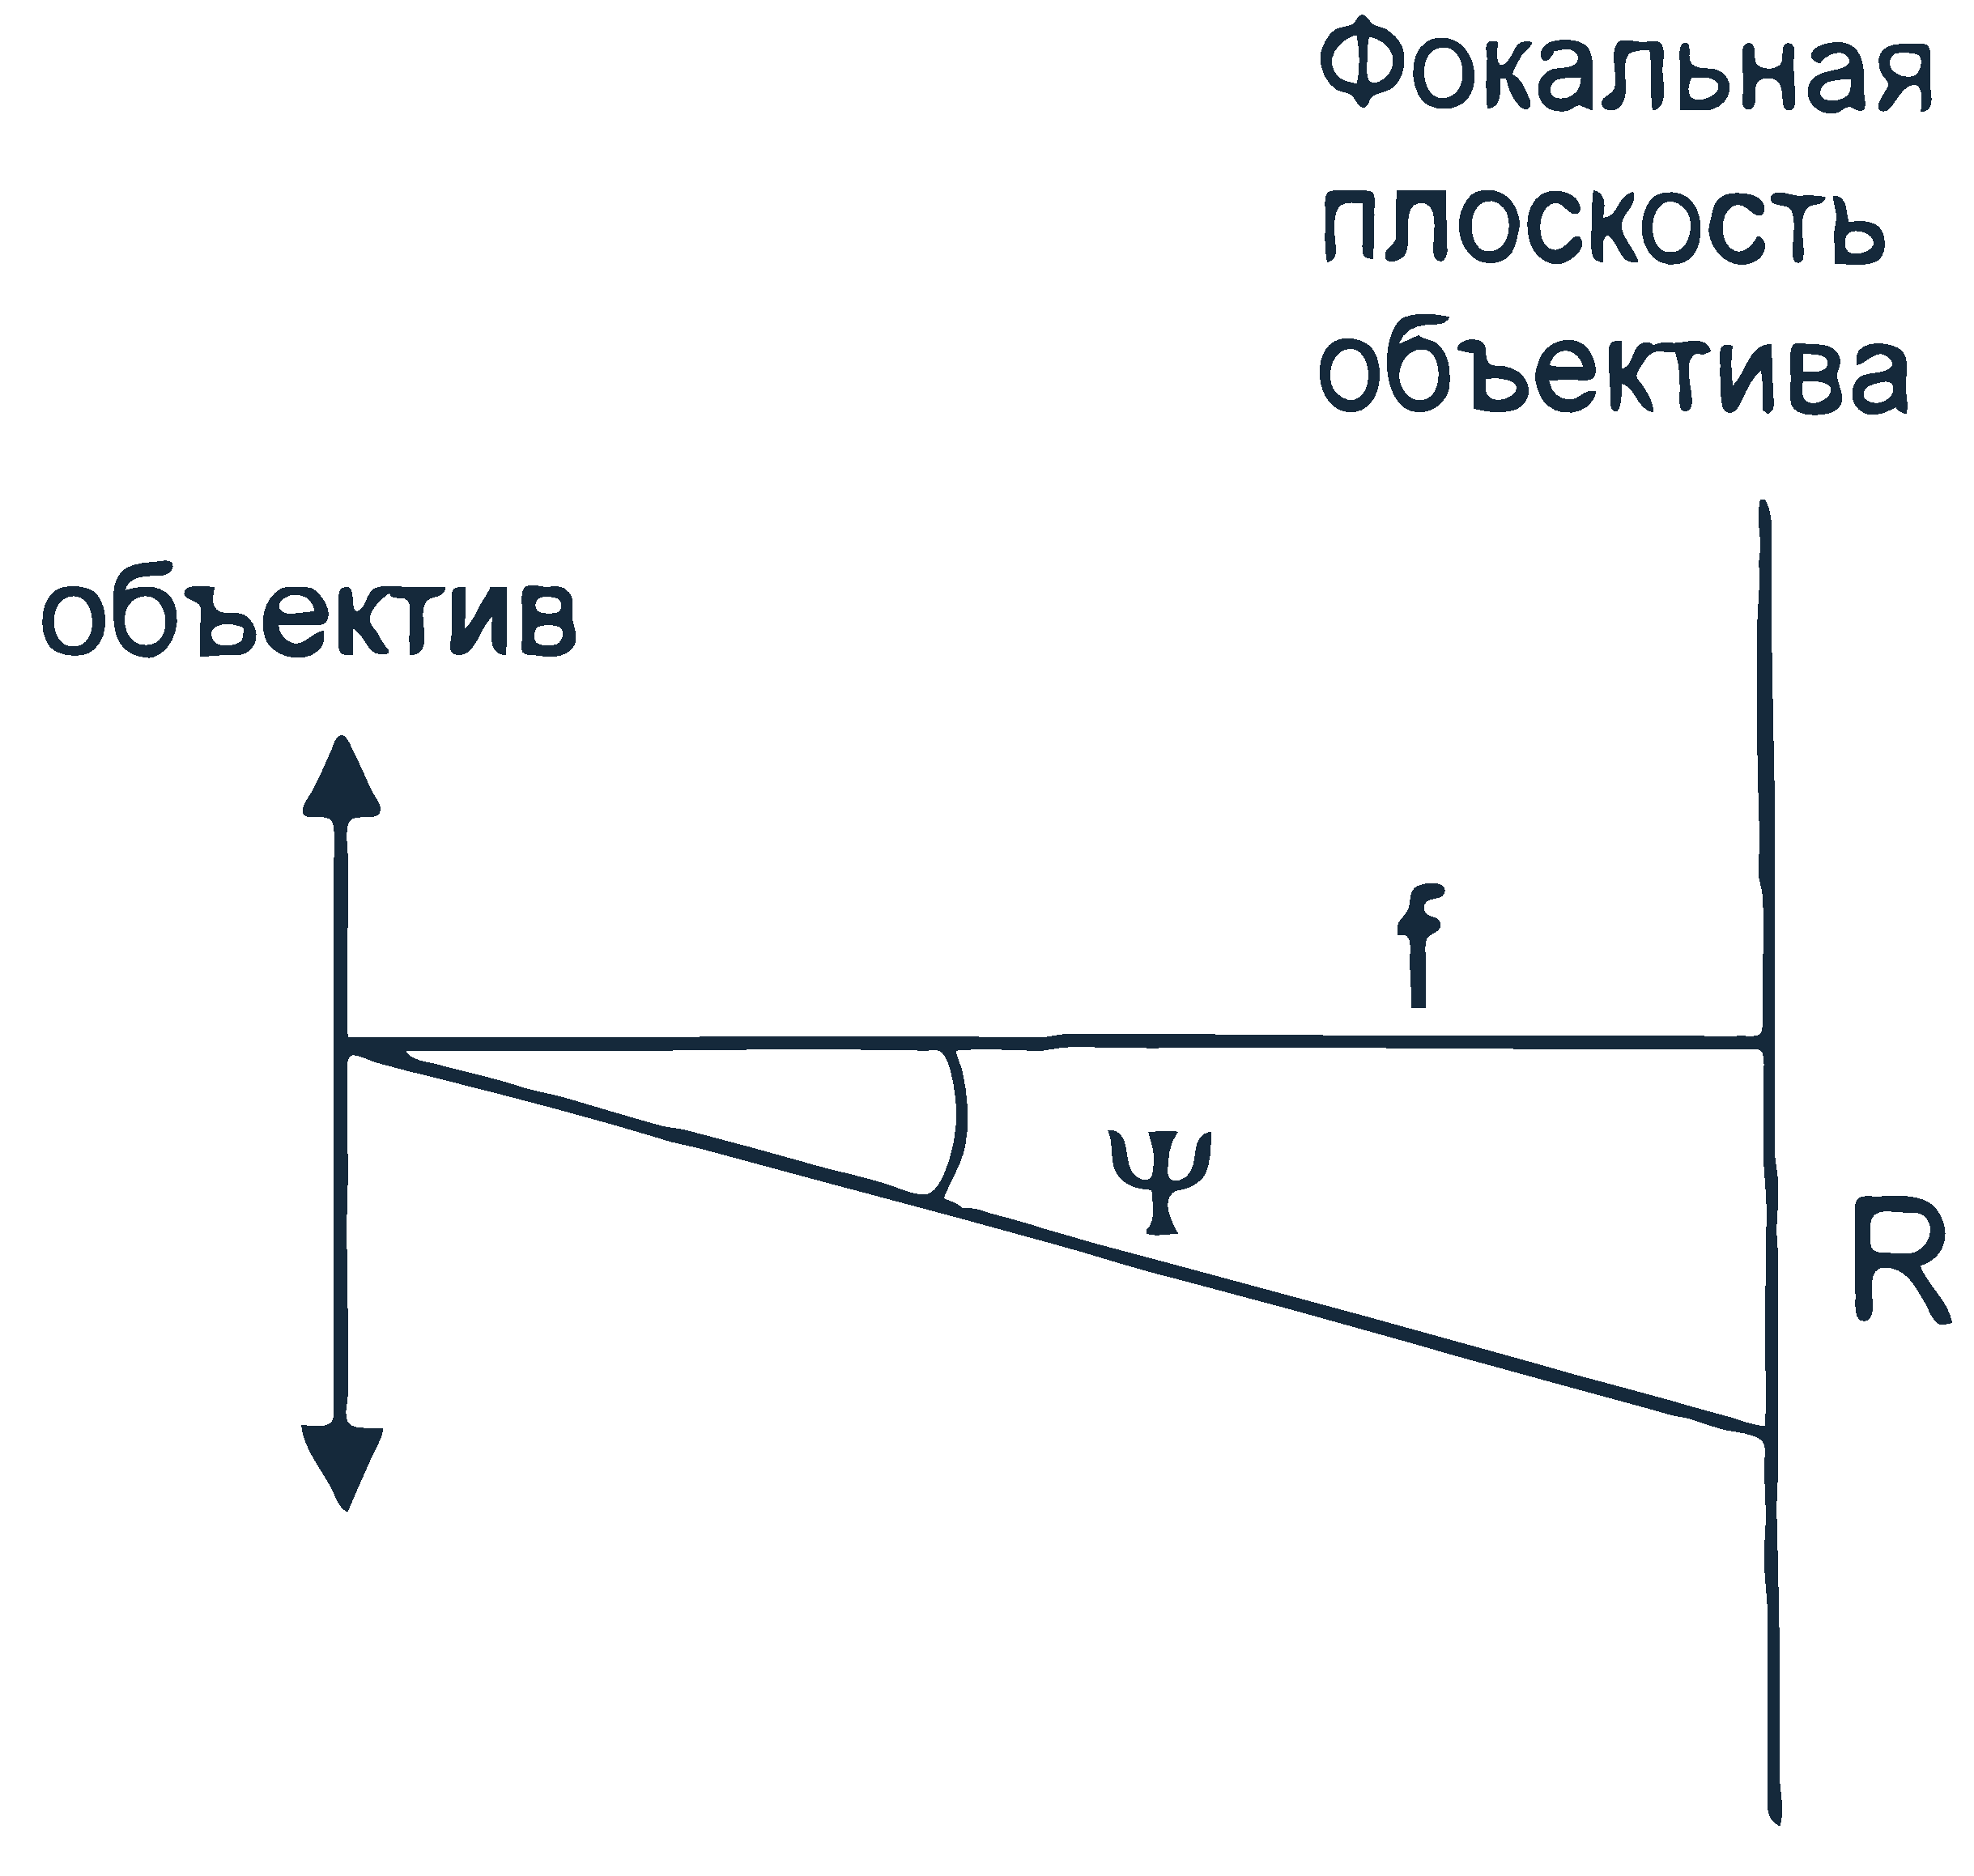
\includegraphics[width=0.5\linewidth]{fig/fig10}
	\caption{К расчету радиуса колец Фабри-Перо}
	\label{fig:10}
\end{figure}

% \begin{wrapfigure}{h}{0.4\textwidth}
% 	\centering
% 	\vspace{-50pt}
% 	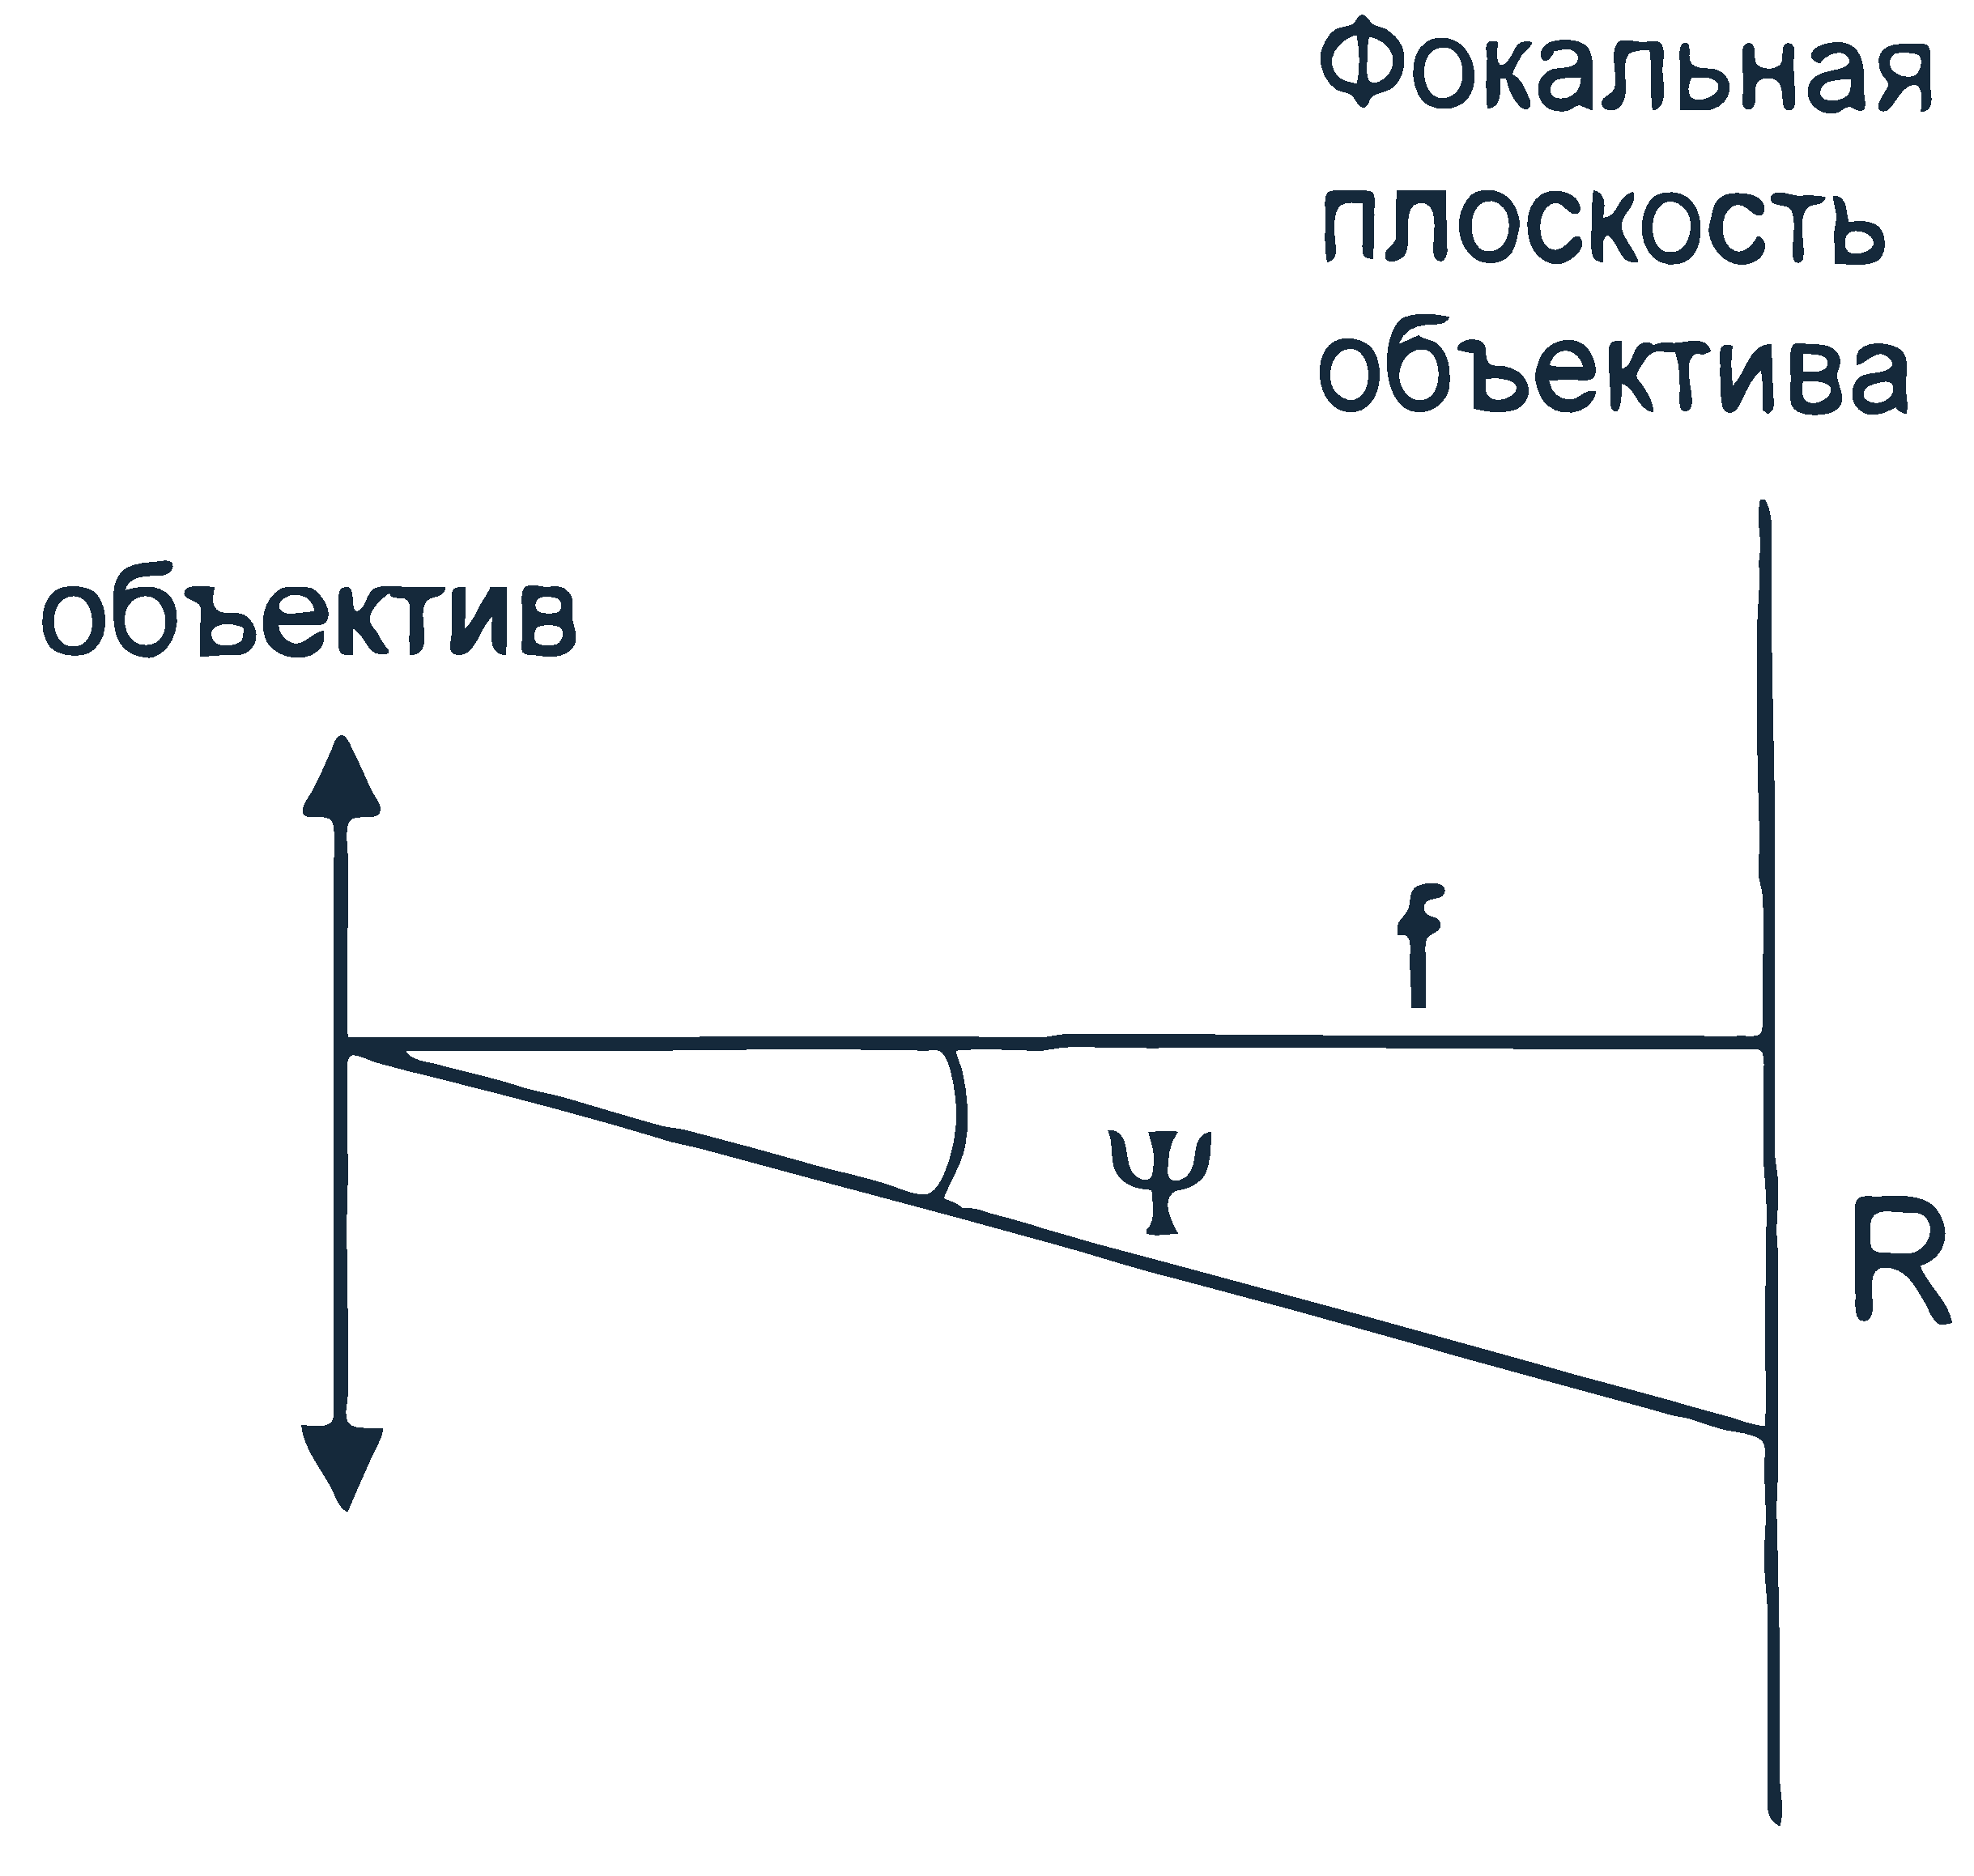
\includegraphics[width=\linewidth]{fig/fig10}
% 	\caption{К расчету радиуса колец Фабри-Перо}\vspace{-45pt}
% 	\label{fig:10}
% \end{wrapfigure}
%рис 10
Величину  разности углов $\delta \Psi_m$ и $\delta \Psi_{\lambda}$ найдем из \ref{eq:24}, которое с учетом малости $\Psi$ примет вид
\begin{gather}
	\label{eq:31}
	1-\frac{\Psi^m}{2}=\frac{m\lambda}{2h}
\end{gather}

Откуда получаем значения 
\begin{gather}
	\label{eq:32}
	\delta \Psi_m=\frac{m\delta \lambda}{2h\Psi_m} и \delta \Psi_{\lambda}=\frac{\lambda}{2h\Psi_{\lambda}}
\end{gather}

Усредняя результаты измерений,получим
\begin{gather}
	\label{eq:33}
 	\langle \Delta R_m \rangle  = f \langle\delta \Psi_m\rangle =f\frac{m\delta \lambda}{2h}  \langle\frac{1}{\Psi_m} \rangle
\end{gather}

Аналогично для
\begin{gather}
	\label{eq:34}
	\langle\Delta R_{\lambda}\rangle  = f \langle\delta \Psi_{\lambda}\rangle =f\frac{\lambda}{2h}  \frac{1}{\Psi_{\lambda}} 
\end{gather}

Из соотношений \ref{eq:33} и \ref{eq:34} с учетом равенства $ \langle\frac{1}{\Psi_m}\rangle = \langle\frac{1}{\Psi_{\lambda}} \rangle$, 
которое следует из того, что углы $\Psi_m$ и $\Psi_{\lambda}$ принимают один и тот же ряд значений, получим формулу для расчета $\delta \lambda$:


% \begin{equation}

% 	\langle \Delta R_{\lambda} \rangle=
% 	\frac{m \delta \lambda}{\lambda},
% \end{equation}

% полагая $m=\frac{2h}{\lambda}$, получим

\begin{equation}
	\label{eq:35}
	\delta \lambda = \frac{\lambda^2}{2h} \frac{\langle \Delta R_m \rangle}{\langle \Delta R_{\lambda}\rangle}
\end{equation}

% Регистрировать данные измерений и производить их обработку удобно, используя таблицу \ref{tab:3}, где $ \langle \Delta \rangle R_m  = \frac{1}{4} \sum^4_{i=1} \Delta R_mi$, $ \langle \Delta  R_{\lambda} \rangle = \frac{1}{3} \sum^3_{i=1} \Delta R_{\lambda i}$
%%%%%%%%%%%%%%%%%%%%%%%%%%%%%%%%%%%%%%%%%%%%%%%%%%%%%%%%%%%%%%%%%%%%%%%%
%!TEX root = ../zeeman.tex
\subsection{Теоретический расчет расщепления линий}
Для 585.25 нм:

$$J \rightarrow J+1$$
$$J_1=0 \Rightarrow M_1=0$$
$$J_2=1 \Rightarrow M_2 =1, 0, -1$$
\begin{figure}[H]
	\centering
	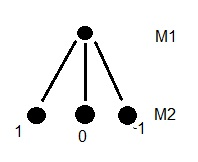
\includegraphics[width=0.3\linewidth]{fig/fig12}
	\caption{}
	\label{fig:fig12}
\end{figure}

Интенсивность:

\begin{tabular}{ | l | l | l | l |}
\hline
$\text{Поперечный эффект}$ & $ $ & $\text{Продольный эффект}$ & $ $ \\ \hline
$0 \rightarrow -1$ & $\frac12$ & $0 \rightarrow -1$ & $1$\\
$0 \rightarrow 0$ & $1$ & $0 \rightarrow 1$ & $1$\\
$0 \rightarrow 1$ & $\frac12$ & $ $ & $ $\\
\hline
\end{tabular}

\begin{tabular}{ | l | l | l | l |}
\hline
$ $ & $0 \rightarrow -1$ & $0 \rightarrow 0$ & $0 \rightarrow 1$ \\
$\Delta \omega$ & $-1$ & $0$ & $1$ \\
$\text{Поляризация}$ & $\sigma$ & $\pi$ & $\sigma$\\
$\text{Интенсивность}$ & $\frac12$ & $1$ & $\frac12$\\
\hline
\end{tabular}

Для 594.48 нм:

$$J \rightarrow J$$
$$J_1=2 \Rightarrow M_1=2,1,0,-1,-2$$
$$J_2=2 \Rightarrow M_1=2,1,0,-1,-2$$
\begin{figure}[H]
	\centering
	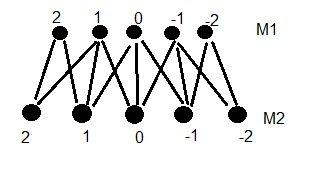
\includegraphics[width=0.3\linewidth]{fig/fig13}
	\caption{}
	\label{fig:fig13}
\end{figure}

Интенсивность:

\begin{tabular}{ | l | l | l | l |}
\hline
$\text{Поперечный эффект}$ & $ $ & $\text{Продольный эффект}$ & $ $ \\ \hline
$2 \rightarrow 2$ & $4$ & $2 \rightarrow 1$ & $2$\\
$2 \rightarrow 1$ & $1$ & $1 \rightarrow 2$ & $2$\\
$1 \rightarrow 2$ & $1$ & $1 \rightarrow 0$ & $3$\\
$1 \rightarrow 1$ & $1$ & $0 \rightarrow 1$ & $3$\\
$1 \rightarrow 0$ & $\frac32$ & $0 \rightarrow -1$ & $3$\\
$0 \rightarrow 1$ & $\frac32$ & $-1 \rightarrow 0$ & $3$\\
$0 \rightarrow 0$ & $0$ & $-1 \rightarrow -2$ & $2$\\
$0 \rightarrow -1$ & $\frac32$ & $-2 \rightarrow -1$ & $2$\\
$-1 \rightarrow 0$ & $\frac32$ & $ $ & $ $\\
$-1 \rightarrow -1$ & $1$ & $ $ & $ $\\
$-1 \rightarrow 2$ & $1$ & $ $ & $ $\\
$-2 \rightarrow -1$ & $1$ & $ $ & $ $\\
$-2 \rightarrow -2$ & $4$ & $ $ & $ $\\
\hline
\end{tabular}

\begin{tabular}{ | l | l | l | l | l | l | l | l | l |}
\hline
$ $ & $2 \rightarrow 2$ & $2 \rightarrow 1$ & $1 \rightarrow 2$ & $1 \rightarrow 1$ & $1 \rightarrow 0$ & $0 \rightarrow 1$ & $0 \rightarrow 0$ & $0 \rightarrow -1$ \\ 
$\Delta \omega$ & $0$ & $\frac32$ & $-\frac32$ & $0$ & $\frac32$ & $-\frac32$ & $0$ & $\frac32$\\ 
$\text{Поляризация}$ & $\pi$ & $\sigma$ & $\sigma$ & $\pi$ & $\sigma$ & $\sigma$ & $\pi$ & $\sigma$\\
$\text{Интенсивность}$ & $4$ & $1$ & $1$ & $1$ & $\frac32$ & $\frac32$ & $0$ & $\frac32$ \\
\hline
\end{tabular}

\begin{tabular}{| l | l | l | l | l | l | l | l |}
\hline
$-1 \rightarrow 0$ & $-1 \rightarrow -1$ & $-1 \rightarrow -2$ & $-2 \rightarrow -1$ & $-2 \rightarrow -2$\\
$-\frac32$ & $0$ & $\frac32$ & $-\frac32$ & $0$\\
$\sigma$ & $\pi$ & $\sigma$ & $\sigma$ & $\pi$\\
$\frac32$ & $1$ & $1$ & $1$ & $4$\\
\hline
\end{tabular}

Для 607.4 нм:

$$J \rightarrow J+1$$
$$J_1=0 \Rightarrow M_1=0$$
$$J_2=1 \Rightarrow M_1=1,0,-1$$
\begin{figure}[H]
	\centering
	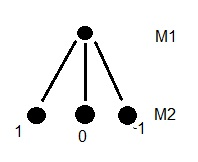
\includegraphics[width=0.3\linewidth]{fig/fig12}
	\caption{}
	\label{fig:fig14}
\end{figure}
Интенсивность:

\begin{tabular}{ | l | l | l | l |}
\hline
$\text{Поперечный эффект}$ & $ $ & $\text{Продольный эффект}$ & $ $ \\ \hline
$0 \rightarrow -1$ & $\frac12$ & $0 \rightarrow -1$ & $1$\\
$0 \rightarrow 0$ & $1$ & $0 \rightarrow 1$ & $1$\\
$0 \rightarrow 1$ & $\frac12$ & $ $ & $ $\\
\hline
\end{tabular}

\begin{tabular}{ | l | l | l | l |}
\hline
$ $ & $0 \rightarrow 1$ & $0 \rightarrow 0$ & $0 \rightarrow -1$ \\
$\Delta \omega$ & $-\frac32$ & $0$ & $\frac32$ \\
$\text{Поляризация}$ & $\sigma$ & $\pi$ & $\sigma$\\
$\text{Интенсивность}$ & $\frac12$ & $1$ & $\frac12$\\
\hline
\end{tabular}

Для 638.3 нм:

$$J \rightarrow J$$
$$J_1=1 \Rightarrow M_1=1,0,-1$$
$$J_2=1 \Rightarrow M_1=1,0,-1$$
\begin{figure}[H]
	\centering
	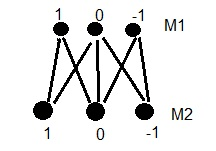
\includegraphics[width=0.3\linewidth]{fig/fig14}
	\caption{}
	\label{fig:fig15}
\end{figure}

Интенсивность:

\begin{tabular}{ | l | l | l | l |}
\hline
$\text{Поперечный эффект}$ & $ $ & $\text{Продольный эффект}$ & $ $ \\
$1 \rightarrow 1$ & $1$ & $1 \rightarrow 0$ & $1$\\
$1 \rightarrow 0$ & $\frac12$ & $0 \rightarrow 1$ & $1$\\
$0 \rightarrow 1$ & $\frac12$ & $0 \rightarrow -1$ & $1$\\
$0 \rightarrow 0$ & $0$ & $-1 \rightarrow 0$ & $1$\\
$0 \rightarrow -1$ & $\frac12$ & $ $ & $1$\\ 
$-1 \rightarrow 0$ & $\frac12$ & $ $ & $1$\\
$-1 \rightarrow 1$ & $1$ & $ $ & $ $\\
\hline
\end{tabular}

\begin{tabular}{ | l | l | l | l | l | l | l | l |}
\hline
$ $ & $1 \rightarrow 1$ & $1 \rightarrow 0$ & $0 \rightarrow 1$ & $0 \rightarrow 0$ & $0 \rightarrow -1$ & $-1 \rightarrow 0$ & $-1 \rightarrow -1$\\ 
$\Delta \omega$ & $-1$ & $\frac12$ & $-\frac32$ & $0$ & $\frac32$ & $-\frac12$ & $1$\\ 
$\text{Поляризация}$ & $\pi$ & $\sigma$ & $\sigma$ & $\pi$ & $\sigma$ & $\sigma$ & $\pi$\\
$\text{Интенсивность}$ & $1$ & $\frac12$ & $\frac12$ & $0$ & $\frac12$ & $\frac12$ & $1$ \\
\hline
\end{tabular}

\subsection{Наблюдение нормального эффекта Зеемана}
На примере линии 585.25 нм.
Характер поляризации компонент при поперечном эффекте:
\begin{figure}[H]
	\centering
	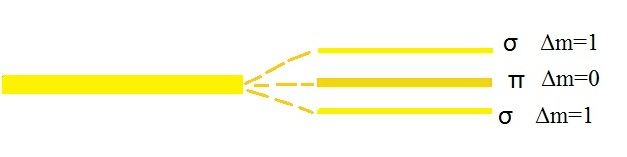
\includegraphics[width=0.5\linewidth]{fig/fig15}
	\caption{}
	\label{fig:fig16}
\end{figure}

Расщепление в поперечном эффекте при значении магнитного поля $H=6100 \text{ эрстед} (1.8 A)$.
\begin{figure}[H]
	\centering
	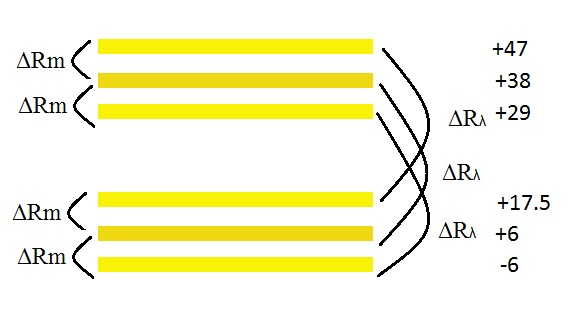
\includegraphics[width=0.5\linewidth]{fig/fig16}
	\caption{}
	\label{fig:fig17}
\end{figure}

Удельный заряд электрона $\frac{e}{m} = \frac{2c^2d\lambda}{\lambda^2 H}$

$\frac{e}{m}_{\text{прак}} = 0.12\cdot10^{18}$, $\frac{e}{m}_{\text{теор}} = 0.52\cdot 10^{18}$.

Разрешающая способность ИФП  при $H=4400 \text{ эрстед} (1 A)$ ($\rho=0.89, m_i=m_0=\frac{2h}{\lambda}$)

$$R_{\text{теор}}=\frac{m_i \pi \sqrt{\rho}}{1-\rho}= 368 900$$
$$R_{\text{прак}}=\frac{\omega}{\Delta \omega}= 82 200$$ 

\subsection{Изучение аномального эффекта Зеемана}
На примере линии 607.4 нм.
Характер поляризации компонент при поперечном эффекте:
\begin{figure}[H]
	\centering
	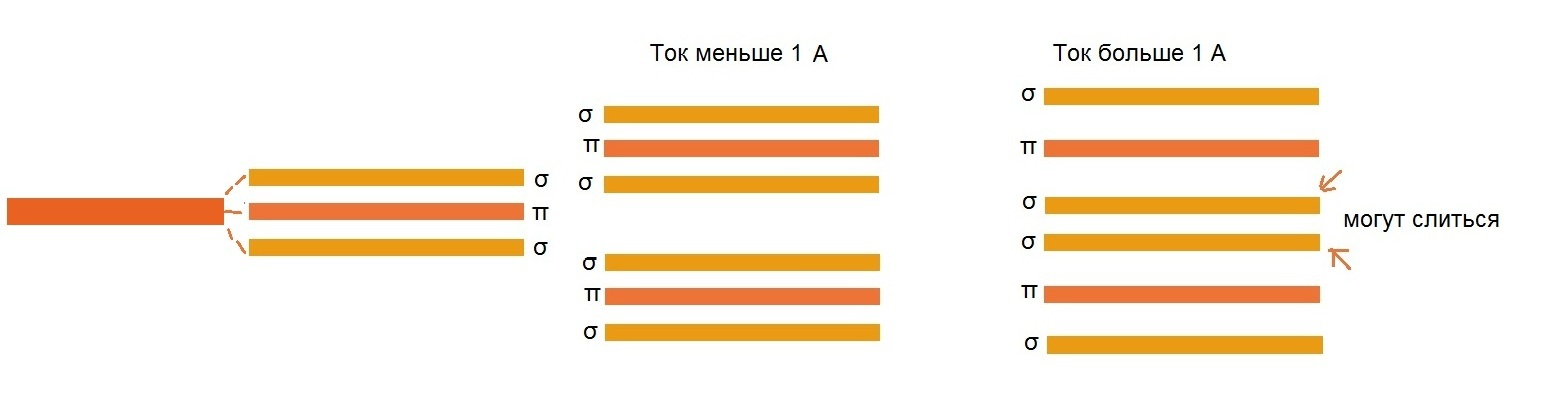
\includegraphics[width=\linewidth]{fig/fig17}
	\caption{}
	\label{fig:fig18}
\end{figure}

Расщепление в поперечном эффекте при значении магнитного поля $H=4400 \text{ эрстед} (1 A)$.
\begin{figure}[H]
	\centering
	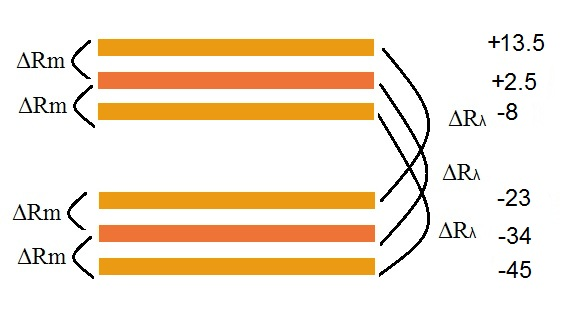
\includegraphics[width=0.5\linewidth]{fig/fig18}
	\caption{}
	\label{fig:fig19}
\end{figure}

разность g-факторов: $1.8 \pm 0.1$.

\subsection{Изучение аномального зеемановского расщепления при наличии более чем трех разрешаемых прибором компонент}
На примере линии 638.3 нм.
\begin{figure}[H]
	\centering
	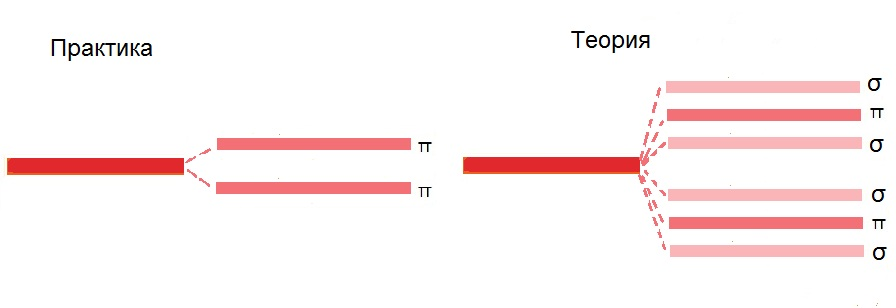
\includegraphics[width=0.8\linewidth]{fig/fig19}
	\caption{}
	\label{fig:fig20}
\end{figure}

Расщепление компонент
\begin{figure}[H]
	\centering
	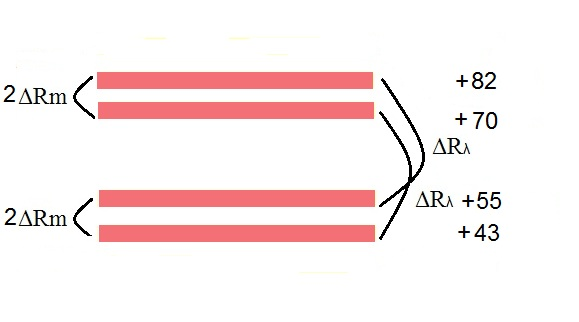
\includegraphics[width=0.5\linewidth]{fig/fig20}
	\caption{}
	\label{fig:fig21}
\end{figure}

разность g-факторов: $1.35 \pm 0.1$.

\subsection{Изучение аномального эффекта Зеемана в условиях частичного разрешения компонент}
На примере линии 594.48 нм.
\begin{figure}[H]
	\centering
	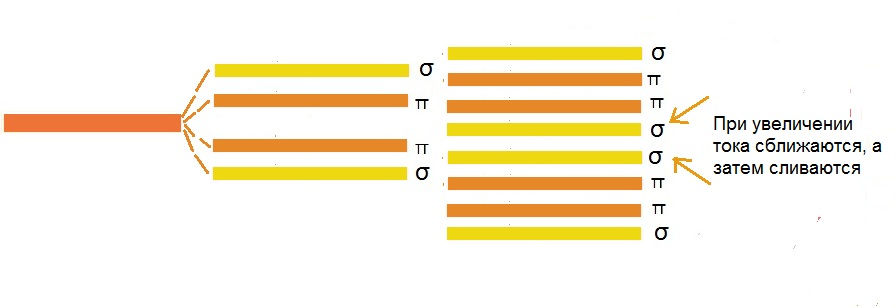
\includegraphics[width=0.8\linewidth]{fig/fig21}
	\caption{}
	\label{fig:fig22}
\end{figure}

Ток, при котором полосы еще различимы $I=2.35 A$. 

\section{Вывод}
В ходе эксперимента изучена теория простого и сложного эффектов Зеемана, исследован характер поляризации компонент в поперечном магнитном поле. Получено значение удельного заряда электрона $\frac{e}{m}_{\text{прак}} = 0.12\cdot10^{18}$, совпадающего по порядку с теоретическим. Оценена разрешающая способность ИФП $R_{\text{прак}}=\frac{\omega}{\Delta \omega}= 82 200$. Определены разности g-факторов для случая аномального эффекта. 


\end{document}